\documentclass{article}

\usepackage[export]{adjustbox}
\usepackage{amsfonts}
\usepackage{amsmath}
\usepackage{amssymb}
\usepackage[utf8]{inputenc}
\usepackage[sorting=none,block=ragged,style=numeric-comp]{biblatex}
\addbibresource{main.bib}
\usepackage{caption}
\usepackage{dsfont}
\usepackage{dirtytalk}
\usepackage{eqparbox}
\usepackage{fancyhdr}
\usepackage{float}
\usepackage[T1]{fontenc}
\usepackage{geometry}
\geometry{a4paper}
\usepackage{graphicx}
\usepackage{hhline}
\usepackage{hyperref}
\usepackage{listings}
\usepackage{mathtools}
\usepackage{multirow}
\usepackage{ragged2e}
\usepackage{subcaption}
\usepackage{titlesec}
\usepackage[table,xcdraw]{xcolor}

\newcommand\alignsymbols[2][c]{\mathrel{\eqmakebox[S][#1]{$#2$}}{}}

\DeclareMathOperator*{\argmax}{arg\,max}
\DeclareMathOperator*{\argmin}{arg\,min}

\setcounter{secnumdepth}{4}
\titleformat{\paragraph}
{\normalfont\normalsize\bfseries}{\theparagraph}{1em}{}
\titlespacing*{\paragraph}
{0pt}{3.25ex plus 1ex minus .2ex}{1.5ex plus .2ex}

\titleformat{\section}[display]
  {\normalfont\bfseries}{}{0pt}{\Large}

\title{Exploration of joint deconvolution algorithms for omic data}
\author{Vadim \textsc{Bertrand}}
\date{}
\makeatletter
    \let\thetitle\@title
    \let\theauthor\@author
    \let\thedate\@date
\makeatother

\definecolor{dark}{RGB}{22,75,94}
\definecolor{lightgrey}{rgb}{.90,.90,.90}
\definecolor{codegreen}{rgb}{0,0.6,0}
\definecolor{codegray}{rgb}{0.5,0.5,0.5}
\definecolor{codepurple}{rgb}{0.58,0,0.82}
\definecolor{backcolour}{rgb}{0.95,0.95,0.92}

\lstdefinestyle{mystyle}{
    backgroundcolor=\color{backcolour},
    commentstyle=\color{codegreen},
    keywordstyle=\color{magenta},
    numberstyle=\tiny\color{codegray},
    stringstyle=\color{codepurple},
    basicstyle=\footnotesize,
    breakatwhitespace=false,
    breaklines=true,
    captionpos=b,
    keepspaces=true,
    numbers=left,
    numbersep=5pt,
    showspaces=false,
    showstringspaces=false,
    showtabs=false,
    tabsize=2
}
\lstset{style=mystyle}

\hypersetup{
    colorlinks=true,
    linkcolor=black,
    filecolor=magenta,
    urlcolor=blue,
    citecolor=blue,
}

\pagestyle{fancy}

\begin{document}
\newgeometry{
 top=20mm,
 bottom=20mm,
 left=20mm,
 right=20mm
}
\begin{titlepage}
    \noindent
	\begin{minipage}{0.5\textwidth}
        
\includegraphics[width=0.61\textwidth,left]{logo/logo_timc}
	\end{minipage}
	\begin{minipage}{0.5\textwidth}
        
\includegraphics[width=0.75\textwidth,right]{logo/logo_im2ag}
	\end{minipage}\\[1.5 cm]

    \begin{center}
        {\Large Université Grenoble Alpes - IM2AG\\[.5 cm]
        Master 2 Mathématiques et Applications,\\
        parcours Statistique et Science des Données (SSD)}\\[1.5 cm]

        \textsc{\LARGE Internship report}
        \\[.5 cm]
        \large realized at TIMC, Grenoble\\[.2 cm]
        March 6 - Sept. 1, 2023\\[1.5 cm]

	    \rule{\linewidth}{0.2 mm} \\[1 cm]
	    {\huge \bfseries \thetitle}\\[.7 cm]
	    \rule{\linewidth}{0.2 mm} \\[1.5 cm]

    	{\Large \theauthor}\\[1.5 cm]
    \end{center}

    \noindent
	\begin{minipage}{0.5\textwidth}
        \RaggedRight \large
        \textbf{TIMC supervisors} \\
        Elise \textsc{Amblard} \\
        Magali \textsc{Richard}
	\end{minipage}
	\begin{minipage}{0.5\textwidth}
        \RaggedLeft \large
        \textbf{Academic supervisor} \\
        Jean-François \textsc{Coeurjolly}
	\end{minipage}
\end{titlepage}
\restoregeometry
\pagebreak

\section*{Acknowledgments}

First of all, I would like to thank the head of my Master's program, Jean-François Coeurjolly, for his role in coordinating internships and centralizing offers, including the one to which I responded. 
This greatly facilitated the process of finding this internship opportunity. \\
I would also like to express my gratitude to the academic jury members, Jean-François Coeurjolly and Rémy Drouilhet, who will read this report and attend my defense. \\

The entire MAGe team has been very welcoming, and it's worth noting that they are also quite skilled in baking delicious pastries and cakes for Tuesday mornings! \\
Finding the appropriate ingredients, recipe, and tasters for MB deconvolution proved to be more challenging.
However, I am grateful that Elise supervised my on this task, granting me substantial freedom, engaging in fruitful discussions about the problems I encountered, and providing valuable insights into the biological questions I had. \\

Finally, thanks a lot to Magali for providing me with this internship opportunity and following its progress during her leave.
I also feel very privileged to have had the chance to attend not only one but two conferences during this period! 
The experience of crafting a poster introducing my work and presenting it at these occasions has been truly educational.

\newpage

\tableofcontents

\newpage

\section{Context}\label{sec:context}

I completed this internship as a conclusion to my second year of master's.
During my first year of master's, I became quite interested in high-dimensional problems and their applications to biological questions.
This interest led me to work under the supervision of Elise Amblard and Magali Richard in the \textit{Modèles et Algorithmes pour la Génomique} (MAGe) team at TIMC (\textit{Recherche \textbf{T}ranslationnelle et \textbf{I}nnovation en \textbf{M}édecine et \textbf{C}omplexité}) on the \textbf{Exploration of joint deconvolution algorithms for omic data}.

TIMC is a highly multidisciplinary laboratory, conducting research in the field of biotechnologies for health.
The MAGe team focuses more closely on developing models and methods for the analysis of omic data in order to address biological, ecological, and clinical questions. \\

My internship is part of the Acacia project, coordinated by Magali Richard, which focuses on Pancreatic Ductal AdenoCarcinoma (PDAC), one of the most lethal cancer types with a 5-year survival rate of less than $10\%$ \cite{bengtsson_2020_rate}.
The analysis of omic data has made it possible to produce classifications of cancer patients, enabling better management of their disease \cite{moffitt_2015_stratification, puleo_2018_stratification}.
However, these classifications only take into account inter-tumoral heterogeneity, disregarding intra-tumoral heterogeneity, which plays an important role in the development of cancer.

Acacia's clinical objective is therefore to propose a new classification of PDAC that takes into account intra-tumor heterogeneity.
Methodologically, we plan to use multi-omic data from bulk tumor samples and develop algorithms for deconvolving cell types (their proportions is a proxy to quantify intra-tumor heterogeneity).

\subsection{Omic data}\label{subsec:omic-data}

Omic data refers to large-scale datasets (meaning that the number of features is orders of magnitude larger than the number of samples) measuring various types of biological characteristics: genomic, epigenomic, transcriptomic, proteomic, etc...
These datasets provide valuable insights about the structure, function, and regulation of genes, proteins, and other biomolecules, and hence about the functioning of cells, organs, or organisms.
Omic data can be measured either on the whole tissue (referred to as bulk) or on a cell (referred to as single-cell). In our work, we will focus on bulk data.
In the scope of Acacia, we have access to the transcriptome and methylome from in vitro generated PDAC tumors. \\

Transcriptome data records the level of expression of all genes by measuring the number of mRNA copies per gene.
In this context, \say{expressed} means that a gene contributes to the production of proteins or RNA molecules.
Gene expression levels are not constant over time and are regulated based on the cell's type and its surroundings: other cells or chemical messengers.
Consequently, researchers analyze transcriptome data to identify differentially expressed genes and gain insight into cellular processes, developmental stages, and disease mechanisms. 
Transcriptome data is typically generated using RNA sequencing (RNA-seq) or microarrays. 
The output of those technologies is a matrix displaying the raw counts of all RNA molecules over the samples measured.

Methylome data, on the other hand, focuses on a chemical modification of the DNA molecule known as DNA methylation. 
Methylation data provides information about the presence or absence of a methyl group at specific regions of the genome (referred to as CpG sites). 
A methyl group prevents the transcription of genes upon binding to the CpG site upstream of those genes.
By analyzing methylation patterns, researchers can identify epigenetic changes associated with various biological processes, including development, aging, and disease. 
Methylation data also offers potential biomarkers for disease diagnosis, prognosis, and therapeutic targets \cite{teodoridis_2004_epigenetic}.
Techniques like bisulfite sequencing or methylation arrays are commonly employed to generate methylation data. 
Two units of measurement are mostly used:
\begin{itemize}
    \item Beta-value: it represents the proportion of methylated cytosines for a given CpG site and ranges from 0 to 1,
    \item M-value: the logit-transformation of the Beta-value.
\end{itemize}

By integrating these two omics, also referred to as blocks, one can hope to leverage information of different nature on biological systems and thus improve their understanding (see \cite{ebrahim_2016_multi} for example).
More specifically, this can benefit the deconvolution task.

\subsection{Tumor heterogeneity}\label{subsec:tumor-heterogeneity}

As shown in Figure \ref{fig:pdac_tumor}, tumors are heterogeneous ecosystems, composed of cancer cells and host cells (also called stromal cells).
The predominant cell type in PDAC tumors is the malignant pancreatic ductal cell.
These cells are characterized by uncontrolled growth and division, leading to tumor formation.
Within the PDAC tumor microenvironment, one can also find cancer-associated fibroblasts (CAFs), which support tumor growth and invasion, as well as immune cells, such as T cells, macrophages, or dendritic cells. The immune system has an ambiguous role in tumor progression, sometimes restraining tumor growth, sometimes supporting it.

\begin{figure}[ht]
    \centering
    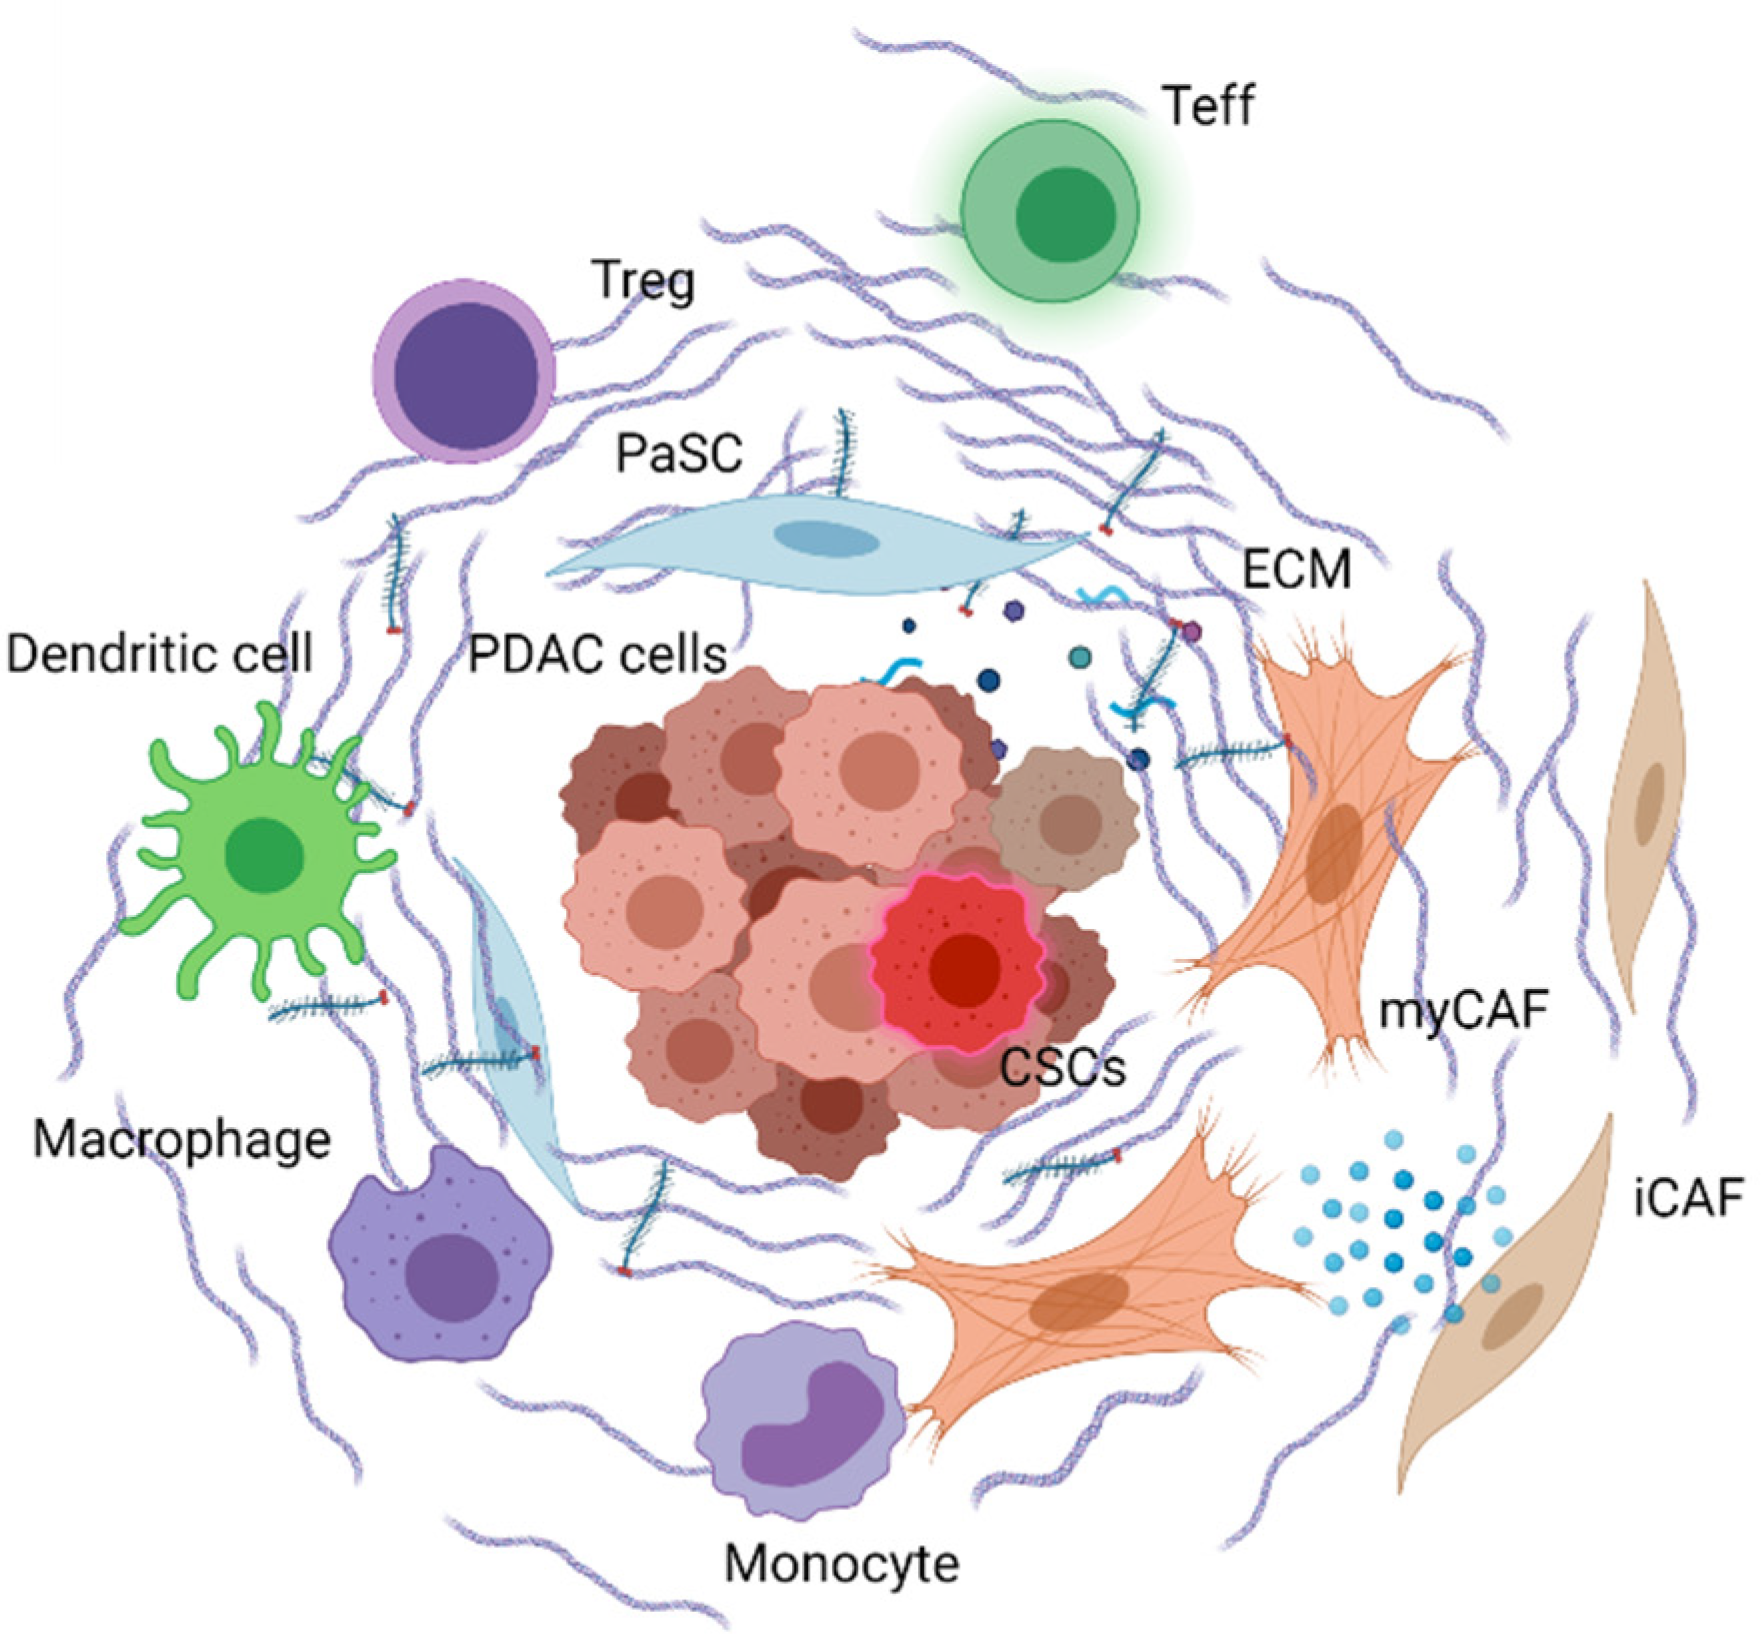
\includegraphics[height=6cm,width=\textwidth,keepaspectratio]{fig/pdac_tumor.png}
    \caption{Cell types present in PDAC tumors, contributing to their heterogeneous composition (from \cite{truong_2021_pancreatic}).}
    \label{fig:pdac_tumor}
\end{figure}

There are two types of tumor heterogeneity:
\begin{itemize}
    \item Inter-tumor heterogeneity, which refers to the differences between patients,
    \item Intra-tumor heterogeneity, which refers to the differences in cellular composition within the tumor itself.
\end{itemize}

Omic data have been used to discriminate patients and produce PDAC cancer classifications \cite{moffitt_2015_stratification, puleo_2018_stratification}, paving the way for better diagnostics and treatments in the future.
Such classifications focus on inter-tumor heterogeneity and only take into consideration the most abundant cancer cell type, disregarding intra-tumor heterogeneity.

Omic data can also be used to quantify intra-tumor heterogeneity through the estimation of the proportions of the different cell types displayed in the tumor, and thus propose finer cancer classifications.
Using single-cell omic data, one can directly quantify the proportions of the cell types within the tumor microenvironment.
However, single-cell data is much more expensive and less often collected in the clinic than bulk data from which estimating cell types proportions is done using deconvolution methods.

\subsection{Principles of cell type deconvolution}\label{subsec:cell-type-deconvolution}

In signal processing, deconvolution refers to the recovery of individual sources from their mixed record.
The same concept can be applied to omic data. \\

We have bulk omic tumor samples (bulk expression matrices $D_{\text{RNA}}$ and $D_{\text{MET}}$).
Rather than gene expression itself, we are interested in the cell types proportions within each tumor (the proportion matrix $A$). 
They are linked by cell type expression profiles (reference matrices $T_{\text{RNA}}$ and $T_{\text{MET}}$) via:
$$
\underset{G \times S}{D} = \underset{G \times K}{T} \times \underset{K \times S}A
$$
with $G$ the number of features in matrix $D$, $S$ the number of samples and $K$ the number of cell types. \\

Deconvolution methods can be separated into two large families: supervised and unsupervised.

The supervised approach requires the $T$ matrix along with $D$ to estimate $A$. 
The quality of the reference matrix is key to the performance of deconvolution. 
It also implies to know beforehand the cell types expected to be present in the samples.

On the other hand, unsupervised methods only need $D$, and estimate both $T$ and $A$. 
While it is more flexible, a major disadvantage has been the difficulty to identify the cell types retrieved during deconvolution, as well as to determine $K$.

Some deconvolution techniques are specific to MET or RNA bulk data, based on each block's own characteristics. \\

I will briefly mention below top-performing supervised and unsupervised deconvolution algorithms \cite{avila_2020_benchmarking, titus_2017_review}.

\subsubsection{Supervised methods}\label{subsubsec:supervised-methods}

First of all, we should note that even when assuming that $T$ is known, $A$ cannot be calculated simply using the Ordinary Least Square (OLS) formula $\widehat{A} = T^{-1} \times D$ because inverting $T$ is often an ill-posed problem, and most of all, OLS does not enforce the two constraints: 
\begin{align}
A_{k,s} \in [0, 1] \text{, } \forall k,s \\
\sum_{k=1}^K A_{k,s} = 1 \text{, } \forall s
\end{align}

However, several deconvolution methods taking into account those constraints are based on OLS:
\begin{itemize}
    \item OLS, or Robust Linear Regression (RLR), or penalized linear regression, followed by a rectified linear unit (ReLU) function, and column-wise normalization,
    \item Non-Negative Least Squares (NNLS), followed by column-wise normalization,
    \item DeconRNASeq \cite{DeconRNASeq} and WISP \cite{WISP}, which directly solve the optimization problem including the two constraints using Quadratic Programming.
\end{itemize}

Other algorithms, such as CIBERSORT \cite{CIBERSORT}, are based on Support Vector Machine (SVM) followed by a ReLU function and column-wise normalization.

Finally, some methods rely on a Bayesian approach to directly sample the columns $\widehat{A_{s}}$ from the posterior distribution $p(A_{s} | D_{s}, T)$.
BayesPrism \cite{BayesPrism} employs Gibbs sampling to do so, while the faster version InstaPrism \cite{InstaPrism} implements a fixed-point algorithm.

\subsubsection{Unsupervised methods}\label{subsubsec:unsupervised-methods}

Two classes of algorithms are mainly used in the unsupervised framework: Independent Component Analysis (ICA) and Non-negative Matrix Factorization (NMF).
The major conceptual difference between the two is that ICA makes the assumption that the produced factors are independent, and it does not enforce the non-negative and convex constraints. \\

The independence hypothesis in the ICA leads to hard-to-interpret results because the cell types are biologically not independent, while factors are often a linear combination of the cell types \cite{rahmani_2018_bayescce}.
Additionally, constraints on the values of the proportion matrix are poorly integrated into ICA. 
Nevertheless, DeconICA \cite{DeconICA} enables the estimation of $A$ and $T$ simultaneously using ICA.

On the other hand, NMF faces the challenge of non-uniqueness in its reconstruction, as current algorithms solving NMF only guarantee convergence to a local minimum.
Several methods based on NMF have been developed, most of which estimate $A$ and $T$ alternatively using different flavours of constrained OLS, known as Alternating Least Square (ALS).
Among these methods, notable ones include NMF \cite{DECONnmf}, RefFreeEWAS \cite{RefFreeEWAS}, MeDeCom \cite{MeDeCom}, and EDec \cite{EDec}.

\subsubsection{Feature selection}\label{subsubsec:optional-feature-selection}

The deconvolution task is made more complex by the high number of features (ranging from 10k to 800k), be it genes or CpGs.
Therefore, some methods can benefit from a preliminary feature selection step, especially slow ones.
We considered the following feature selection strategies:
\begin{itemize}
    \item Highly Variable Features (referred to as HVG): retain the features with the largest variance, or coefficient of variation,
    \item TOAST \cite{TOAST}: iteratively restrict features to the ones that are cell-type specific, determined thanks to ICA.
\end{itemize}

\subsection{Multi-omics integration strategies}\label{subsec:multi-omics-integration-strategies}

The current state-of-the-art methods mentioned in \ref{subsec:cell-type-deconvolution} are referred to as Simple-Block (SB) methods, meaning they solely utilize one type of omic data.
As their performances remain unsatisfying, especially for unsupervised methods, there is hope to enhance the estimation of cell types proportions by using a Multi-Block (MB) approach, considering that multi-omic data provide more biological information \cite{ebrahim_2016_multi}. \\

In the data integration task, there are three modes: vertical (samples are common across blocks -our study case), horizontal (features are common across blocks), or diagonal (no shared elements across blocks). 
When vertically integrating several blocks, there are four options:
\begin{itemize}
    \item Early integration: blocks are fused before the downstream task is performed. The most common approach is to concatenate features from the different modalities,
    \item Intermediate integration: blocks' features are projected to a shared latent space in which the downstream task is solved. Recently, several methods have been proposed, employing Optimal Transport (OT) \cite{uniPort} or graph embedding representations \cite{MultiMAP, GLUE, MultiXrank},
    \item Late integration: the downstream task is performed on each block and the results obtained are averaged (using the mean, for example),
    \item Serial integration: the task of interest is performed successively on the first block, then on the second while using the results of the task from the first block.
\end{itemize}

\subsection{Constructing fair and comprehensive benchmarks}\label{subsec:constructing-robust-benchmarks}

When developing new methods, it is important to compare them to already existing ones.
In order to publish them, it is almost mandatory that they demonstrate improved performance.
This raises questions about the implementation and fine-tuning of the methods tested against, the metrics used, and the datasets analyzed for comparison, as they can introduce various optimistic biases \cite{buchka_2021_evaluation}.

For instance, fair and comprehensive benchmarks should consider several evaluation metrics (or judges) measuring different desirable characteristics of the methods (or candidates), such as raw performance, performance stability, or computational cost.
Next, it is important to design an appropriate score aggregation strategy to rank the candidates while preserving the contributions of the different categories of scores.
Assessing the statistical significance of the difference in aggregated scores also seems to be an important step toward credible benchmarking studies.

\section{Proposed approach}\label{sec:proposed-approach}

In the following section, I will first detail the benchmark pipeline that allows to compare MB and SB methods.
Then, I will go through the MB approaches I implemented during the internship.

Sections \ref{subsubsec:data-generation} and \ref{subsubsec:scoring-ranking} present the developments previously undertaken by the team and to whom my contribution has been quite limited.
Sections \ref{subsubsec:statistically-significant-performance-improvement}, \ref{subsec:explored-multi-omics-algorithms} and \ref{subsec:running-experiments} relate to the work I directly conducted.

\subsection{Our benchmark setting}\label{subsec:our-benchmark-setting}

As detailed in Table \ref{tab:datasets}, our benchmark operates on four datasets: three simulated (in silico), and one real (in vitro).
Among the simulated ones, two feature cell types found in pancreatic cancer (one PDAC and one general pancreatic cancer), and the last one features cell types found in breast cancer.
The real dataset corresponds to in vitro generation of PDAC tumors.

\begin{table}[ht]
\centering
\caption{Summary of the employed datasets.}
\label{tab:datasets}
\begin{tabular}{l|l|l}
id & type & cancer \\ \hline
dBREAST & simulated & breast \\
dPANCREAS & simulated & pancreatic \\
lot1\_simu & simulated & PDAC \\
lot1\_real & in vitro & PDAC
\end{tabular}
\end{table}

When considering the combinations of the different feature selection strategies (three in total: no selection, HVG, and TOAST), the omic block used (again three: SB -RNA and MET-, or MB), and deconvolution methods (around 20), we evaluated a total of $C \approx 190$ deconvolution candidates.

\subsubsection{Data generation}\label{subsubsec:data-generation}

In order to benchmark on a large diversity of samples, and to have access to reliable \say{ground truth} proportions, we simulated $N=3$ datasets in addition to the in vitro one we have.
Each dataset is composed of two paired blocks: the RNA one, holding transcriptomic data, and the MET one, containing the matching methylome data. \\

The same procedure has been followed to simulate RNA and MET blocks, only the reference matrix $T$ changed.
In both cases the simulation process required a reference matrix $T$ obtained in vitro (i.e. a real measure).
Those reference matrices provide genes expression profiles per cell type for the RNA block, and CpG site proportion of methylated cytosines profiles per cell type for the MET block. \\

We then need to account for biological and technical noise when generating proportion and expression matrices.

Biological noise is usually modelled by sampling proportions from a Dirichlet distribution, the multivariate generalization of the beta distribution.
For every dataset, we sampled $M=10$ proportion matrices $A^{n,m}$: $A^{n,m}_{s} \sim \text{Dir}(\alpha)$, with $\alpha = \alpha_1, ..., \alpha_K$ the shape vector of the $K$ cell types, and $s \in \{1,...,S=120\}$, meaning that each simulated proportion matrix contains the cell types proportions of 120 tumor samples.
Note that the proportion matrix $A^{n,m}$ is the same for the MET and RNA blocks for a given sampling and dataset.

The Dirichlet distribution is a very convenient proxy to express cell types proportions since its support $x_1, \cdots, x_K$ is such that $x_k \in [0,1]$, and $\sum_{k=1}^K x_k = 1$.
In addition, $\alpha$ can be chosen proportional to prior knowledge on the cell types mix in real samples, multiplied by a factor controlling the dispersion around those typical proportions. 
The dispersion factor mimics the biological noise, whose magnitude can be modulated.

By multiplying the $T^n$ in vitro reference matrix with the simulated $A^{n,m}$ matrix, we obtained $N\times M=30$ simulated $D^{n,m}$ expression matrices for each modality (RNA or MET) to which we added a technical noise:
$$D^{n,m} = T^{n} \times A^{n,m} + \epsilon^{n,m}$$
with $\epsilon^{n,m}$ sampled from a Negative Binomial distribution for the methylome block and from a Gaussian distribution for the transcriptome one.

Table \ref{tab:datasets_detail} summarizes the characteristics of each dataset.

\begin{table}[ht]
\centering
\caption{Benchmark datasets characteristics.}
\label{tab:datasets_detail}
\begin{tabular}{l|c|c|c|c|c|c|c|c|c}
& \multicolumn{5}{c|}{Number of replicates} & \multicolumn{4}{c}{Matrices dimensions} \\ \hhline{~|---------|}
& \multicolumn{2}{c|}{$D$} & \multicolumn{2}{c|}{$T$} & \multirow{2}{*}{$A$} & \multirow{2}{*}{$S$} & \multicolumn{2}{c|}{$G$} & \multirow{2}{*}{$K$} \\ \hhline{~|--|--|~~|--|~|}
dataset & RNA & MET & RNA & MET & & & RNA & MET & \\ \hline
dBREAST & 10 & 10 & 1 & 1 & 10 & 120 & 19k & 35k & 4 \\
dPANCREAS & 10 & 10 & 1 & 1 & 10 & 120 & 28k & 772k & 5  \\
lot1\_simu & 10 & 10 & 1 & 1 & 10 & 120 & 21k & 825k & 9  \\
lot1\_real & 1 & 1 & 1 & 1 & 1 & 30 & 21k & 825k & 9 
\end{tabular}
\end{table}

\subsubsection{Scoring and ranking}\label{subsubsec:scoring-ranking}

\paragraph{Desired properties}\label{paragraph:desired-properties}

Ranking candidates based on judges' preferences is a common task in various domains such as politics and economics.
For instance, we can envision the candidates as politicians and the judges as citizens.
In this context, social sciences and game theory have extensively studied various election strategies.
More recently, researchers from the field of Machine Learning (ML) have also started examining ranking processes used to benchmark competing algorithms \textendash the candidates\textendash \space on multiple tasks or criteria \textendash the judges\textendash. \\

Several theoretical criteria characterizing ranking processes' robustness to candidates or judges perturbation, and its winner's (good) properties have been inherited from game theory and social sciences:
\begin{itemize}
    \item Majority criterion: the winner should be the candidate ranked first by more than 50\% of the judges (winner property),
    \item Condorcet criterion: the winner should be the Condorcet winner, which is the candidate who would win in all pairwise rankings against the other candidates, if such a candidate exists (winner property),
    \item Consistency criterion: if ranking on arbitrary partitions of the judges yields the same result, ranking on the entire set of judges should also lead to the same result (judges perturbation),
    \item Participation criterion: removing a judge favoring candidate $i$ over candidate $j$ should only increase the final rank of $j$ with respect to $i$ (judges perturbation),
    \item Independence of Irrelevant Alternatives (IIA) criterion: the final ranking between two candidates should only depend on the individual preferences between those two (candidates perturbation).
\end{itemize}

While these theoretical properties can serve as a basis to choose a fair ranking strategy, evaluating and satisfying them strictly is in practice complicated \cite{arrow_1950_voting, gibbard_1973_voting}.
Therefore, relying solely on theoretical properties is not sufficient to assess the consistency of a ranking process.
To remedy this, Pavao et al. \cite{pavao_2021_judging} proposed corresponding empirical criteria.
We selected the followings for a characterization of our ranking strategies:
\begin{itemize}
    \item Average rank of the winner: normalized averaged rank across all judges (winner property),
    \item Condorcet rate: the frequency at which the winner is ranked first in all pairwise comparisons against the other candidates (winner property),
    \item Generalization: correlation between an out-of-bag judge's ranking and the ranking of the remaining set of judges, computed by bootstrap (judges perturbation).
\end{itemize}

\paragraph{Aggregation of evaluation metrics}\label{paragraph:evaluation-metrics-aggregation}

We have decided to evaluate the deconvolution candidates using $J=12$ metrics sorted into three performance categories to compromise between the quality of the deconvolution and its computational cost:
\begin{itemize}
    \item Raw performance: mean of the Root-Mean-Square Error (RMSE), Mean Absolute Error (MAE) and Pearson correlations ($r(A, \widehat{A})$, $\frac{1}{K} \sum_{k=1}^K r(A_{k.},  \widehat{A_{k.}})$ and $\frac{1}{S} \sum_{s=1}^S r(A_{.s}, \widehat{A_{.s}})$),
    \item Stability: standard deviations of RMSE, MAE and Pearson correlations across datasets' replicates,
    \item Computational cost: mean computation time and its associated standard deviation across datasets' replicates.
\end{itemize}
Upon computing the individual scores (the judges) of the evaluated deconvolution pipelines (the candidates) on the different datasets (extending the set of judges), we obtain a metric tensor $\mathbf{S}$ of size $C \text{ (candidates)} \times J \text{ (judges)} \times N \text{ (datasets)}$.

There is a large number of ways to aggregate those metrics in order to rank deconvolution pipelines. 
But as mentioned earlier some are likely to be more robust and consistent than others. 
Taking into consideration the theoretical criteria introduced previously, we designed the following aggregation strategy, denoted $\mathcal{F}: \mathbb{R}^{C \times J \times N} \longrightarrow \mathbb{R}^C$:
\begin{enumerate}
    \item Pre-process $\mathbf{S}$:
    \begin{enumerate}
        \item Normalize scores in the $[0, 1]$ range for a given judge and dataset:
        $$\mathbf{S}^{01}_{c,j,n} = \Phi\left(\frac{\mathbf{S}_{c,j,n}' - \overline{\mathbf{S}_{.,j,n}'}}{\widetilde{\mathbf{S}_{.,j,n}'}}\right), ~~c \in \{1,...,C\}, ~j \in \{1,...,J\}, ~n \in \{1,...,N\}$$
        \item Transform the metrics such that $1$ is the best score:
        $$
        \mathbf{S}^{101}_{c,j,n} = 
        \begin{cases}
          1 - \mathbf{S}^{01}_{c,j,n} & \text{if} ~j \in \{\text{metrics}\}_{1 ~\text{is worst}} \\
          \mathbf{S}^{01}_{c,j,n} & \text{otherwise}
        \end{cases}
        , ~~c \in \{1,...,C\}, ~j \in \{1,...,J\}, ~n \in \{1,...,N\}
        $$
        \item Average per candidate, score category, and dataset, of all Pearson correlations related scores into a meta Pearson correlation score, yielding $\mathbf{S}^{101'}$ of size $C \times (J'=8) \times N$,
        \item Derive additional tensors $\mathbf{S}^t$ and $\mathbf{S}^r$ from $\mathbf{S}^{101'}$ by computing the TOPSIS similarity \cite{yoon_1981_topsis} and inverse ranks (such that the highest score ranks first).
    \end{enumerate}
    \item Aggregate $\mathbf{S}^{101'}$, $\mathbf{S}^t$ and $\mathbf{S}^r$ separately using the function $\mathcal{F'}: \mathbb{R}^{C \times J' \times N} \longrightarrow \mathbb{R}^C$ (as illustrated in Figure \ref{fig:agg}):
    \begin{enumerate}
        \item Geometric mean of the scores per candidate, score category and dataset, returning a tensor of size $C \times 3 \times N$,
        \item Geometric mean of the scores per candidate and dataset, returning a matrix of size $C \times N$,
        \item Arithmetic mean of the scores per candidate, returning a vector of size $C$,
    \end{enumerate}
    \item Final averaging:
    $$\mathcal{F}(\mathbf{S}) = \frac{\mathcal{F'}(\mathbf{S}^{101'}) + \mathcal{F'}(\mathbf{S}^t) + \mathcal{F'}(\mathbf{S}^r)}{3}$$
\end{enumerate}

\begin{figure}[ht]
    \centering
    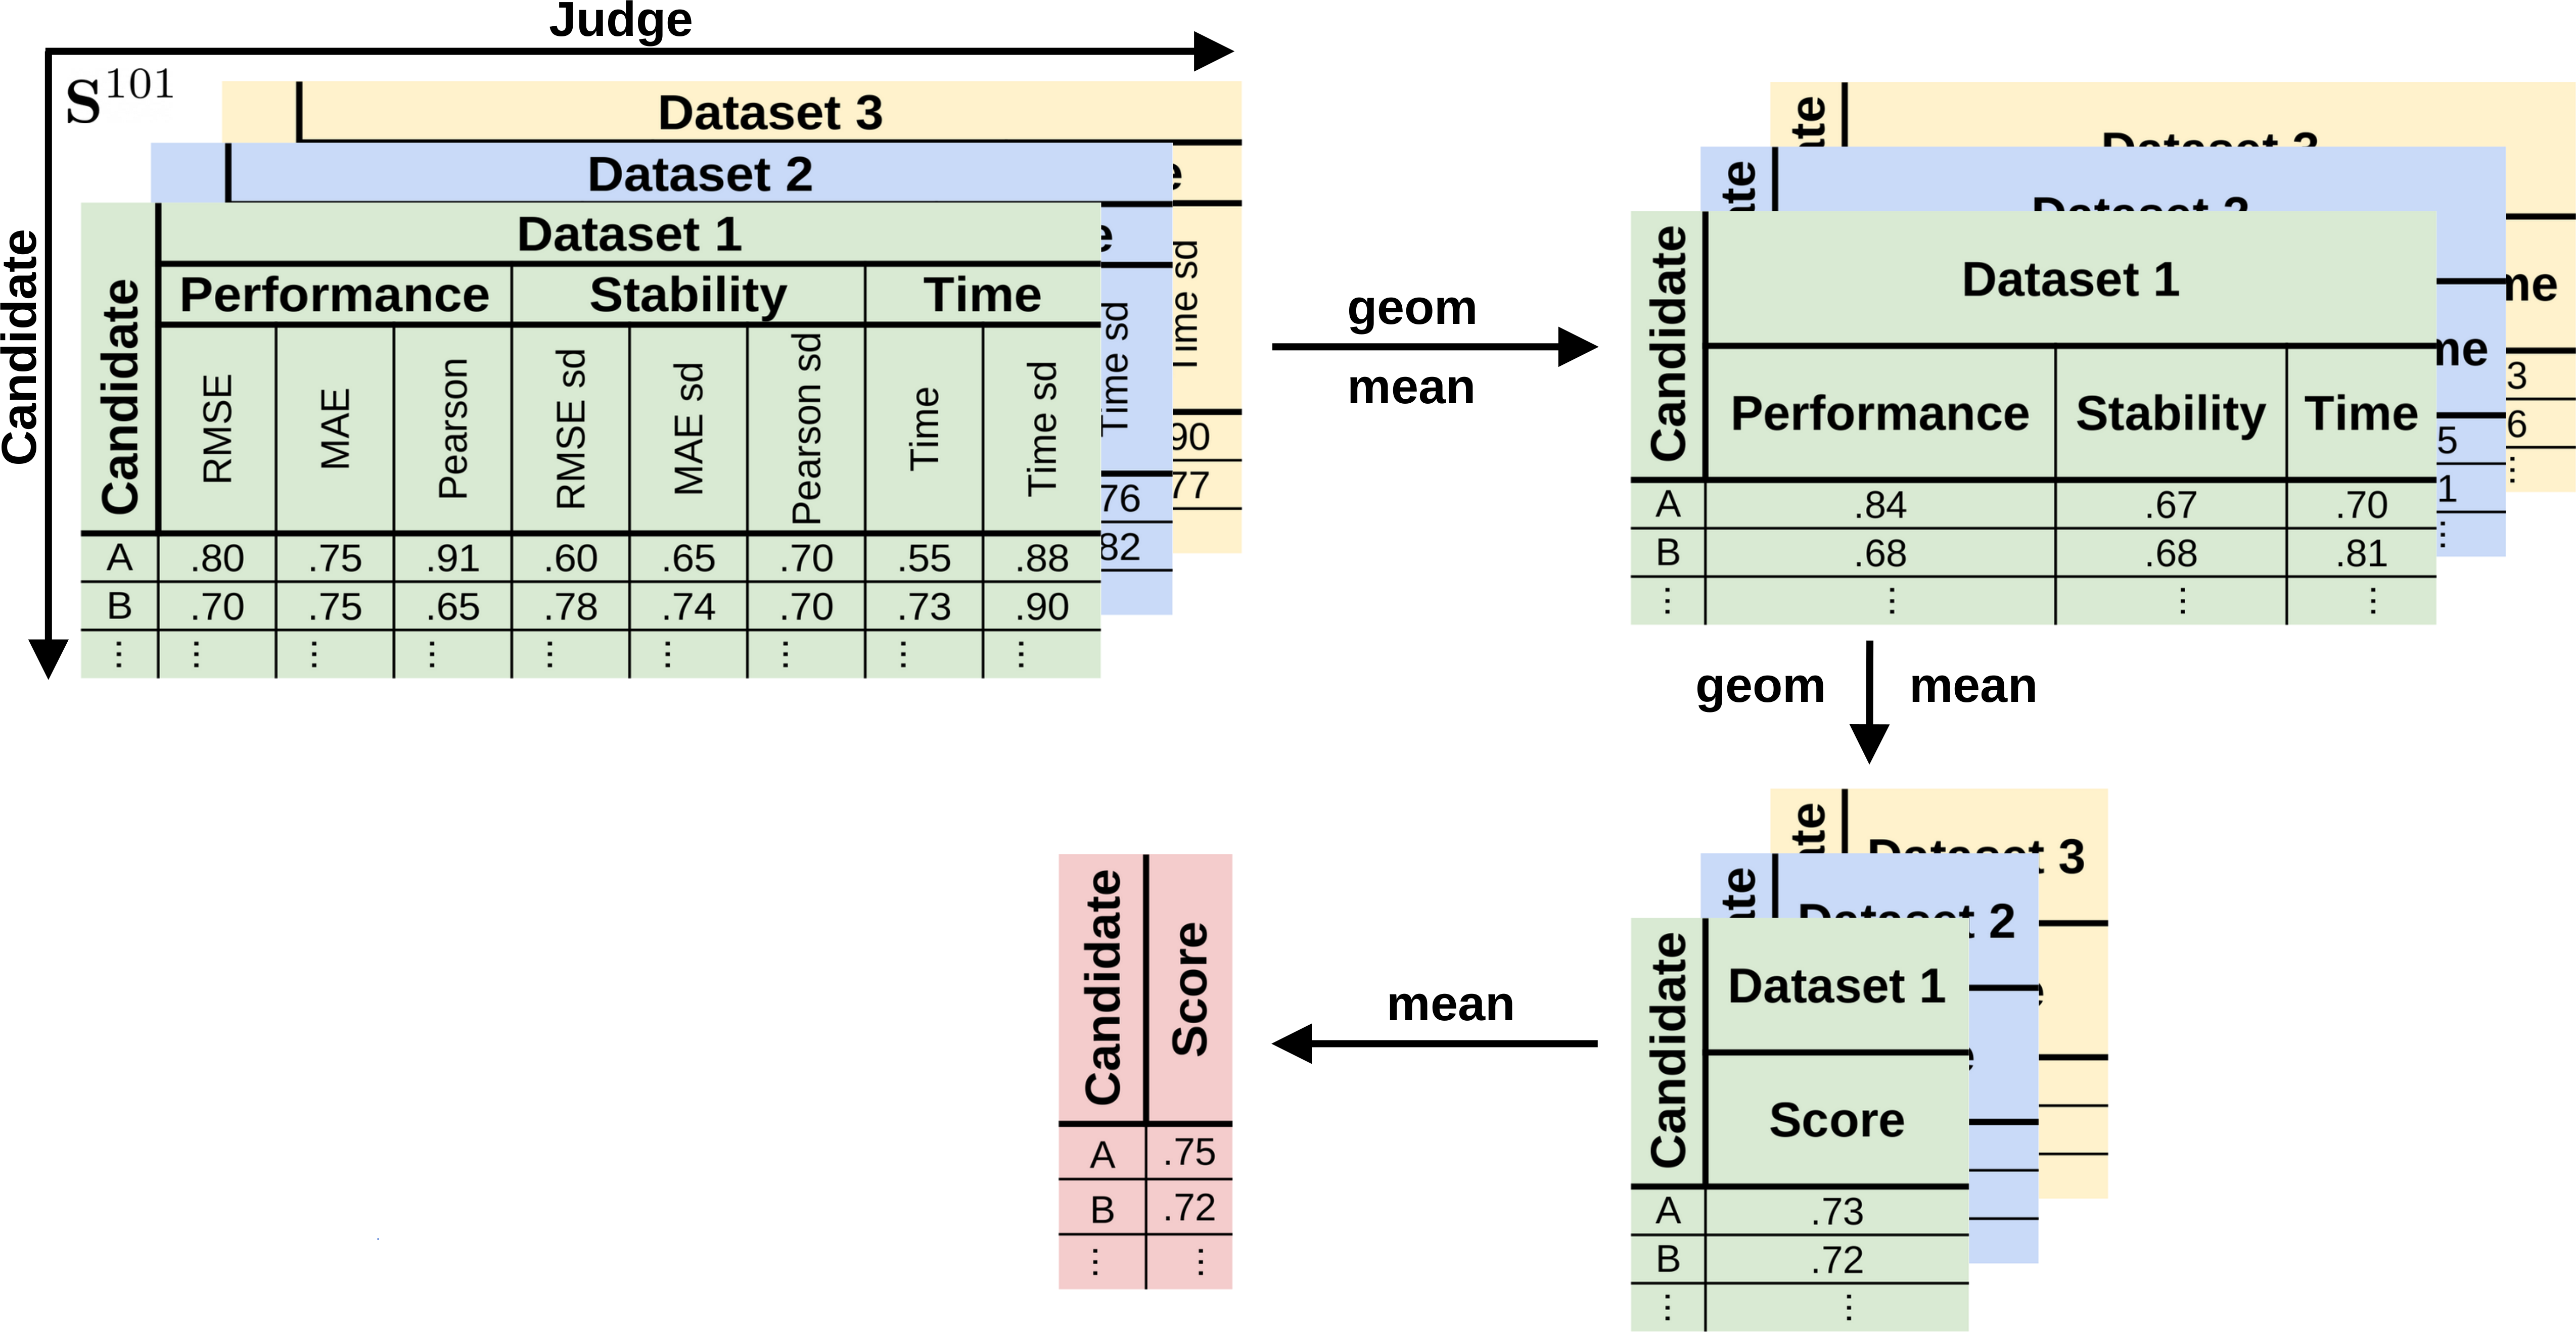
\includegraphics[height=6cm,width=\textwidth,keepaspectratio]{fig/agg.png}
    \caption{Schematic representation of the aggregation function $\mathcal{F'}$.}
    \label{fig:agg}
\end{figure}

\subsubsection{Statistically significant performance improvement}\label{subsubsec:statistically-significant-performance-improvement}

Beside considerations regarding the robustness of ranking processes, it is also of interest to evaluate the significance of difference in the aggregated score between pairs of candidates (top candidates generally).
Due to our complicated aggregation function, using a classical paired Student test to do so would not be satisfying, as it would resort to testing for the simple arithmetic mean of the scores' differences, which is quite different from $\mathcal{F}$. \\

In order to test more accurately for the difference in the aggregated scores, I proposed to use a \say{pairwise} Monte Carlo permutation test.
Under the null hypothesis, the individual scores of two candidates, $c_1$ and $c_2$, are drawn from the same probability distribution, and hence, their final aggregated score expectations are equal.
We consider the one-sided alternative hypothesis that the expectation of $c_1$ aggregated score is larger than that of $c_2$.

By rearranging the observed individual scores, we are able to generate data under the null hypothesis and obtain an empirical distribution of the test statistic under the null hypothesis.
We then reject or accept the null hypothesis based on the empirical quantile of the observed test statistic.

With this setting, the test procedure can be detailed as follows:
\begin{enumerate}
    \item Compute the observed test statistic: $s_0 = \mathcal{F}(\mathbf{S})_{c_1} - \mathcal{F}(\mathbf{S})_{c_2}$,
    \item Repeat $P=1000$ times (see Table \ref{tab:perm_test} for a visual representation):
        \begin{enumerate}
            \item Draw probabilities of permuting two paired metrics: $p_i \sim \mathcal{U}(0,1), ~i \in \{1,...,J*N\}$,
            \item Permute paired metrics:
            $$\mathbf{S}^p_{cjn} = 
            \begin{cases}
              \mathbf{S}_{c_2jn} & \text{if} ~c = c_1 ~\text{and} ~p_{j+J(n-1)} \geq 0.5 \\
              \mathbf{S}_{c_1jn} & \text{if} ~c = c_2 ~\text{and} ~p_{j+J(n-1)} \geq 0.5 \\
              \mathbf{S}_{cjn} & \text{otherwise}
            \end{cases}
            , ~~c \in \{1,...,C\}, ~j \in \{1,...,J\}, ~n \in \{1,...,N\}
            $$
            \item Compute $s_p = \mathcal{F} \left( \mathbf{S}^p \right)_{c_1} - \mathcal{F} \left( \mathbf{S}^p \right)_{c_2}$,
        \end{enumerate}
    \item Compute the $\text{p-value} = \frac{1}{P + 1} (1 + \sum_{p=1}^P \mathds{1}_{s_p \geq s_0})$.
\end{enumerate}

\begin{table}[ht]
\centering
\caption{Permutation procedure outputs example. The red individual scores correspond to scores originally belonging to candidate $c_1$, and the blue ones to candidate $c_2$.}
\label{tab:perm_test}
%\resizebox{\textwidth}{!}{
\begin{tabular}{l|c|
>{\columncolor[HTML]{D9EAD3}}c 
>{\columncolor[HTML]{D9EAD3}}c 
>{\columncolor[HTML]{D9EAD3}}c |
>{\columncolor[HTML]{C9DAF8}}c 
>{\columncolor[HTML]{C9DAF8}}c 
>{\columncolor[HTML]{C9DAF8}}c |
>{\columncolor[HTML]{FFF2CC}}c 
>{\columncolor[HTML]{FFF2CC}}c 
>{\columncolor[HTML]{FFF2CC}}c |
>{\columncolor[HTML]{F4CCCC}}c |
>{\columncolor[HTML]{D0E0E3}}c }
\multicolumn{2}{l|}{} & \multicolumn{3}{c|}{\cellcolor[HTML]{D9EAD3}Dataset 1} & \multicolumn{3}{c|}{\cellcolor[HTML]{C9DAF8}Dataset 2} & \multicolumn{3}{c|}{\cellcolor[HTML]{FFF2CC}Dataset 3} & \multicolumn{2}{l}{\cellcolor[HTML]{FFFFFF}} \\ \hhline{~~|---------|}
\multicolumn{2}{l|}{$p$} & $s_1$ & ... & $s_{12}$ & $s_1$ & ... & $s_{12}$ & $s_1$ & ... & $s_{12}$ & $\mathcal{F}_p$ & $s_p$ \\ \hline
& {\color[HTML]{CB0000} $c_1$} & {\color[HTML]{CB0000} .80} & {\color[HTML]{CB0000} ...} & {\color[HTML]{CB0000} .88} & {\color[HTML]{CB0000} .76} & {\color[HTML]{CB0000} ...} & {\color[HTML]{CB0000} .76} & {\color[HTML]{CB0000} .78} & {\color[HTML]{CB0000} ...} & {\color[HTML]{CB0000} .90} & .75 & \cellcolor[HTML]{D0E0E3} \\
\multirow{-2}{*}{0} & {\color[HTML]{3531FF} $c_2$} & {\color[HTML]{3531FF} .70} & {\color[HTML]{3531FF} ...} & {\color[HTML]{3531FF} .90} & {\color[HTML]{3531FF} .74} & {\color[HTML]{3531FF} ...} & {\color[HTML]{3531FF} .82} & {\color[HTML]{3531FF} .71} & {\color[HTML]{3531FF} ...} & {\color[HTML]{3531FF} .77} & {\color[HTML]{333333} .72}                      & \multirow{-2}{*}{\cellcolor[HTML]{D0E0E3}.03} \\ \hline
& {\color[HTML]{CB0000} $c_1$} & {\color[HTML]{3531FF} .70} & {\color[HTML]{CB0000} ...} & {\color[HTML]{CB0000} .88} & {\color[HTML]{CB0000} .76} & {\color[HTML]{CB0000} ...} & {\color[HTML]{CB0000} .76} & {\color[HTML]{CB0000} .78} & {\color[HTML]{CB0000} ...} & {\color[HTML]{3531FF} .77} & .74 & \cellcolor[HTML]{D0E0E3} \\
\multirow{-2}{*}{1} & {\color[HTML]{3531FF} $c_2$} & {\color[HTML]{CB0000} .80} & {\color[HTML]{3531FF} ...} & {\color[HTML]{3531FF} .90} & {\color[HTML]{3531FF} .74} & {\color[HTML]{3531FF} ...} & {\color[HTML]{3531FF} .82} & {\color[HTML]{3531FF} .71} & {\color[HTML]{3531FF} ...} & {\color[HTML]{CB0000} .90} & {\color[HTML]{333333} .73}                      & \multirow{-2}{*}{\cellcolor[HTML]{D0E0E3}.01} \\ \hline
\rotatebox[origin=t]{90}{\,...} & \rotatebox[origin=t]{90}{\,...} & & \rotatebox[origin=t]{90}{\,...} & & & \rotatebox[origin=t]{90}{\,...} & & & \rotatebox[origin=t]{90}{\,...} & & \rotatebox[origin=t]{90}{\,...} & \rotatebox[origin=t]{90}{\,...} \\ \hline
& {\color[HTML]{CB0000} $c_1$} & {\color[HTML]{CB0000} .80} & {\color[HTML]{CB0000} ...} & {\color[HTML]{3531FF} .90} & {\color[HTML]{CB0000} .76} & {\color[HTML]{CB0000} ...} & {\color[HTML]{CB0000} .76} & {\color[HTML]{3531FF} .71} & {\color[HTML]{CB0000} ...} & {\color[HTML]{CB0000} .90} & .74 & \cellcolor[HTML]{D0E0E3} \\
\multirow{-2}{*}{1000} & {\color[HTML]{3531FF} $c_2$} & {\color[HTML]{3531FF} .70} & {\color[HTML]{3531FF} ...} & {\color[HTML]{CB0000} .88} & {\color[HTML]{3531FF} .74} & {\color[HTML]{3531FF} ...} & {\color[HTML]{3531FF} .82} & {\color[HTML]{CB0000} .78} & {\color[HTML]{3531FF} ...} & {\color[HTML]{3531FF} .77} & {\color[HTML]{333333} .71} & \multirow{-2}{*}{\cellcolor[HTML]{D0E0E3}.03}
\end{tabular}
%}
\end{table}

\subsection{Explored multi-omics algorithms}\label{subsec:explored-multi-omics-algorithms}

Having a well defined evaluation framework, we can go further and investigate multi-omics deconvolution approaches.
Late and serial integration timing methods have been developed previously to my internship, therefore I focused on the implementation of early and intermediate integration timing methods.

\subsubsection{Early integration}\label{subsubsec:early-integration}

Early integration refers to fusing the omics before performing the deconvolution task.
In the scope of Acacia, some early methods had already been investigated, in particular, concatenating features of the methylome and transcriptome blocks.
Those attempts did not improve much the deconvolution performance so I experimented with another (rather naive) fusion strategy: the summation of the blocks.

The idea is that when considering the blocks separately, we can represent the supervised deconvolution task as a system of two equations with only one unknown (since the cell types proportions we want to estimate are the same for the two modalities):
$$
\begin{cases}
  D_\text{RNA} = T_\text{RNA} \times A_\text{RNA} \\
  D_\text{MET} = T_\text{MET} \times A_\text{MET}
\end{cases}, \text{ and } A_\text{RNA} = A_\text{MET} \coloneqq A
$$

If the dimensions of the $D$ and $T$ matrices match, we can factorize the system:
$$D_\text{RNA} + D_\text{MET} = (T_\text{RNA} + T_\text{MET}) \times A$$

Usually, it is not the case, as the methylome block has many more features than the transcriptome one (about 750k against 40k).
However, we can easily overcome this by selecting the $G_\text{RNA}$ most variable features of the matrix $D$ from the methylome block ($G_\text{RNA}$ being the number of features of the transcriptome one).

Another point to consider is the different ranges of values of the two blocks: the methylome one displays Beta-values, reals lying in $[0, 1]$; whereas the transcriptome one is made of raw counts, natural numbers (including 0).
After selecting the most variable features of the largest block to obtain expression and reference matrices of the same dimensions and before factorizing the system, we should, therefore, normalize the blocks separately.
For simplicity, I switched here to (column) vector notation:
\begin{equation}
\label{eq:sum}
\begin{split}
    &
    \begin{cases}
      d_1 = T_1 \times a \\
      d_2 = T_2 \times a
    \end{cases} \\
    \alignsymbols{\iff} &
    \begin{cases}
      \frac{d_1 - \mu_1}{\sigma_1} \coloneqq y_1 = \frac{T_1 \times a - \mu_1}{\sigma_1} \\
      \frac{d_2 - \mu_2}{\sigma_2} \coloneqq y_2 = \frac{T_2 \times a - \mu_2}{\sigma_2}
    \end{cases} \\
    \alignsymbols[c]{\Longrightarrow} & y_1 + y_2 = \frac{T_1 \times a - \mu_1}{\sigma_1} + \frac{T_2 \times a - \mu_2}{\sigma_2} \\
    \alignsymbols{\iff} & y_1 + y_2 = \frac{\sigma_2 T_1 \times a + \sigma_1 T_2 \times a - \sigma_2 \mu_1 - \sigma_1 \mu_2}{\sigma_1 \sigma_2} \\
    \alignsymbols{\iff} & \sigma_1 \sigma_2 (y_1 + y_2) + \sigma_2 \mu_1 + \sigma_1 \mu_2 = (\sigma_2 T_1 + \sigma_1 T_2) \times a
\end{split}
\end{equation}
with $\mu$ and $\sigma$ denoting the empirical mean and variance, and the subscripts 1 and 2 referring to RNA and MET.
We note that the left-hand side of the last equality could be simplified by re-injecting $d_1$ and $d_2$, but we want to exhibit the summation of the two blocks after normalization.

Wrapping up, the summation procedure consists of:
\begin{enumerate}
    \item Selecting the most variable features (using the HVG strategy introduced in Section \ref{subsubsec:optional-feature-selection}) of the largest block, such that the dimensions of the matrices $D$ and $T$ match,
    \item Normalizing the blocks separately and factorizing the system following Equation \ref{eq:sum},
    \item Applying a supervised deconvolution method.
\end{enumerate}

The deconvolution methods considered in the last step are all based on OLS:
\begin{itemize}
    \item RLR using the \textbf{R} \textit{MASS} package \cite{MASS} followed by a ReLU function and column-wise normalization,
    \item Constrained RLR using the \textbf{R} \textit{MASS} and \textit{restriktor} packages \cite{MASS, restriktor},
    \item Constrained linear optimization using the \textbf{R} \textit{constOptim} function (with L1, L2 and Jensen-Shannon divergence losses) followed by column-wise normalization,
    \item Quadratic Programming using the \textbf{R} \textit{limSolve} package \cite{limSolve}.
\end{itemize}

Finally, it is interesting to point out that this integration approach does not have any particular biological meaning since the features of the two blocks that are summed are paired randomly.
One could try to incorporate some biological knowledge by summing genes and their corresponding CpG sites.
Additionally, it could be interesting to explore the use of weights when summing to balance the importance of the two blocks.

\subsubsection{Intermediate integration}\label{subsubsec:intermediate-integration}

Intermediate integration seeks to learn a shared latent representation of the blocks and perform the deconvolution task in the latent space.
Interesting Deep Learning (DL)-based integration methods for cancer have recently been proposed \cite{leng_2022_benchmark}, which have led us to investigate that direction.
More precisely, two classes of methods are showing strong performances: Variational Autoencoders (VAE) and Graph Neural Networks (GNN).
Due to their smaller size and ease of use (in short, because GNNs require the adjacency matrix of the graphs), we have decided to focus on a VAE-based integration method, rather than a GNN-based one.
The architectures described in paragraph \ref{paragraph:owo-two-vae} have been implemented in \textbf{Python}, using the \textit{PyTorch} library \cite{Paszke_PyTorch_An_Imperative_2019}.

\paragraph{VAE principles}\label{paragraph:vae-principles}

Since our objective is not to generate new data from our latent space, we will not dive into the mathematical foundations of VAE and their link with variational inference.
We can instead see them as Autoencoders (AE) with a regularized latent space.

AE are composed of one encoder and one decoder, each of them modeled by a Multilayer perceptron (MLP).
The encoder maps the input data to a lower-dimensional latent space, while the decoder attempts to reconstruct the original input data from the latent representation of the encoder.
They can be denoted by the two functions $f_e: \mathbb{R}^I \longrightarrow \mathbb{R}^L$ and $f_d: \mathbb{R}^L \longrightarrow \mathbb{R}^I$.
The encoder and decoder are optimized simultaneously by mini-batch gradient descent to minimize the mean square error (MSE) between the input data and its reconstruction from the latent space: $$(f_e^*, f_d^*) = \argmin_{(f_e, f_d)} \text{MSE}(x, f_d(f_e(x)))$$

Rather than producing a single point, the VAE encoder maps the input data to a probability distribution by learning the parameters describing this distribution.
Often, the prior assumption about the distribution in the latent space is a Gaussian and the encoder can be characterized by two functions $f_\mu: \mathbb{R}^I \longrightarrow \mathbb{R}^L$ and $f_\sigma: \mathbb{R}^I \longrightarrow \mathbb{R}^L$ corresponding to its mean and variance.
Then, the decoder operates on a realization sampled from the latent distribution: $z = f_\mu(x) + f_\sigma(x) \xi \text{, } \xi \sim \mathcal{N}(0, 1)$.
In order to obtain a continuous and structured latent space, a VAE adds an additional Kullback-Leibler divergence term to the loss function, encouraging the latent distribution to be similar to a Gaussian.
The final optimization objective is therefore: 
$$(f_\mu^*, f_\sigma^*, f_d^*) = \argmin_{(f_\mu, f_\sigma, f_d)} \text{MSE}(x, f_d(z)) + \text{KL}(\mathcal{N}(f_\mu(x), f_\sigma(x)), \mathcal{N}(0, 1))$$

In the literature, multi-omics integration is performed by either concatenating the omics features before feeding the VAE \cite{OmiVAE}, or by training as many VAEs as omic blocks and concatenating their means and variances to construct a shared latent space \cite{leng_2022_benchmark}.

\paragraph{OWO-VAE and TWO-VAE}\label{paragraph:owo-two-vae}

Since we are only considering two omics, transcriptome and methylome, I proposed to first consider a VAE encoding from the space of one of the block and decoding to the other one, with the intuition that the learned latent space should capture patterns from both blocks.
I will refer to this type of architecture as OWO-VAE (for OneWayOmics-VAE).
In order to perform end-to-end learning, the deconvolution task is done using a MLP operating on the mean of the latent space distribution and denoted by $g$.
Details about the different parts of the architecture are presented in Table \ref{tab:vae}.
After adding the cross-entropy (CE) term of the deconvolution task and weighting the terms, we obtain the following loss function:
$$
\mathcal{L}_\text{OWO} = \lambda_1 (\text{MSE}(d_2, f_d(z_1)) + \lambda_2 \text{KL}(\mathcal{N}(f_\mu(d_1), f_\sigma(d_1)), \mathcal{N}(0, 1))) + \text{CE}(a, g(\mu_1))
$$
with $\lambda_i$ the weights of the different terms of the loss, $d_1, d_2$ a sample of the two blocks, $z_1$ the draw from the latent space distribution of $d_1$, and $\mu_1$ the mean of the latent space distribution of $d_1$.

\begin{table}[ht]
\centering
\caption{OWO-VAE architecture layers specifications.}
\label{tab:vae}
\resizebox{\textwidth}{!}{\begin{tabular}{l|c|c|c|c|c|c|c|c|c|c|c}
& \multicolumn{4}{c|}{Encoder layers} & \multicolumn{4}{c|}{Decoder layers} & \multicolumn{3}{c}{Deconv layers} \\ \hhline{~|-----------|}
& 1 & 2 & 3 & 4 & 1 & 2 & 3 & 4 & 1 & 2 & 3 \\ \hline
IN & $G$ & 2048 & 512 & 256 & 64 & 256 & 512 & 2048 & 64 & 32 & 16 \\ \hline
OUT & 2048 & 512 & 256 & 64 & 256 & 512 & 2048 & $G$ & 32 & 16 & $K$ \\ \hline
Act. & ReLU & ReLU & ReLU & & ReLU & ReLU & ReLU & sigmoid & ReLU & ReLU & (softmax)
\end{tabular}}
\end{table}

Elaborating on this, I proposed to use two OWO-VAEs in parallel, one encoding from the transcriptome to the methylome, and the other from the methylome to the transcriptome.
The means from the two OWO-VAEs are fused to perform the deconvolution task using the element-wise sum.
I also add a new term to the loss function, pushing the two OWO-VAEs latent space distributions closer.
Inspired by OT multi-omics integration strategies, this term computes the Sinkhorn divergence \cite{cuturi_2013_sinkhorn, feydy_2019_interpolating} (a fast approximation of the Wasserstein distance) between the OWO-VAEs latent space distributions.
In the following, this architecture will be referred to as TWO-VAE (TwoWayOmics-VAE).
Its complete loss function is:
$$
\mathcal{L}_\text{TWO} = \lambda_1 (\mathcal{L}_1  + \mathcal{L}_2) + \lambda_3 \text{SD}(z_1, z_2) + \text{CE}(a, g(\mu))
$$
with:
\begin{equation*}
\begin{split}
    & \mathcal{L}_1 = \text{MSE}(d_2, f_d(z_1)) + \lambda_2 \text{KL}(\mathcal{N}(f_\mu(d_1), f_\sigma(d_1)), \mathcal{N}(0, 1)) \\
    & \mathcal{L}_2 = \text{MSE}(d_1, f_d(z_2)) + \lambda_2 \text{KL}(\mathcal{N}(f_\mu(d_2), f_\sigma(d_2)), \mathcal{N}(0, 1))
\end{split}
\end{equation*}
A visual representation of the TWO-VAE architecture is proposed in Figure \ref{fig:two_vae}.

\begin{figure}[ht]
    \centering
    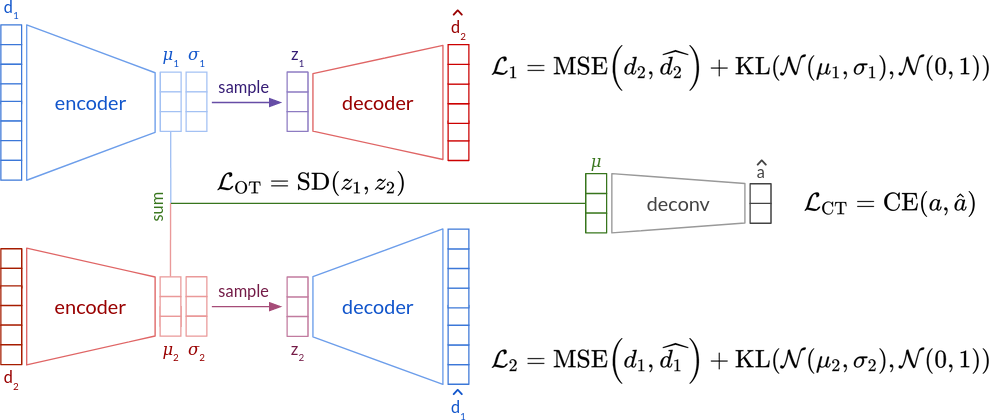
\includegraphics[height=6cm,width=\textwidth,keepaspectratio]{fig/TWO-VAE.png}
    \caption{Overview of the TWO-VAE architecture.}
    \label{fig:two_vae}
\end{figure}

As opposed to the early integration approach described previously, the two architectures belong to the unsupervised family of deconvolution algorithms.

\paragraph{Training the models}\label{paragraph:training-the-models}

Unlike the previous approaches, those models required training.
For each simulated dataset, I created a new set of simulated data, following the procedure described in Section \ref{subsubsec:data-generation}, and randomly divided those sets for training (70\%) and validation (30\%).
The validation set is used to prevent a potential over-fitting during the training procedure.

We decided to build one model for all three datasets, as opposed to one per dataset, in the spirit of having one comprehensive pan-cancer model and not dataset-specific ones.
For this reason, I had to restrict the transcriptome and methylome features to the intersection of the three datasets, resulting in around 20k features for the transcriptome block and 2k for the methylome one.
Originally, methylome data consists of circa 750k features, but the breast reference matrix we are using was produced using a different technology and had only about 35k features, which explains the small size of the intersection.
I also had to consider differences in cell types across the datasets when building the deconvolution part of the model.
We chose to concatenate all the cell types, 18 in total, and set to 0 the proportions of the cell types coming from a dataset other than the dataset of interest.

The gradient descent optimization was performed using the Adam method, with an initial learning rate set to 1e-3 and multiplied by 0.2 whenever the loss computed on the validation set did not decrease for 10 epochs.
Additionally, I set the batch size to 64 samples.

During my initial attempts at training the networks, I encountered the issue of \say{KL vanishing}: the optimizer finds a cheap way to minimize the loss function by focusing on the regularization term of the loss.
This results in the construction of latent space distributions that poorly represent the patterns interesting for reconstruction and, most importantly, deconvolution.
To mitigate this, the \say{sigmoid annealing schedule} has proven to be effective \cite{bowman_2015_generating, fu2_019_cyclical}.
The principle is fairly simple: the weight attached to the regularization term of the loss ($\lambda_2$ in our case) is kept equal to 0 during the first training epochs and then increased to 1 using a logistic function.
The following expression allows controlling the epoch $u_0$ at which the weight starts to increase and the epoch $u_1$ from which it is equal to 1, as well as the steepness of the curve $k$:
$$
\lambda_2(u) =
\begin{cases}
    0 & \text{if} ~u < u_0 \\
    (1 + e^{-k(u - u_{1/2}})^{-1} - (1 + e^{-k(u_0 - u_{1/2}})^{-1} & \text{if} ~u \geq u_0 ~\text{and} ~u < u_{1/2} \\
    0.5 & \text{if} ~u = u_{1/2} \\
    1 + (1 + e^{-k(u - u_{1/2}})^{-1} - (1 + e^{-k(u_1 - u_{1/2}})^{-1} & \text{if} ~u > u_{1/2} ~\text{and} ~u \leq u_1 \\
    1 & \text{otherwise}
\end{cases}
$$
with $u_{1/2} = (u_0 + u_1) / 2$ being the midpoint of the function.

Even though we decided to fix the number and the size of the layers used in the encoder, decoder and deconvolution parts of the network, there are some hyperparameters left to tune.
Since tuning hyperparameters is quite costly, as it requires training from scratch, I \say{only} considered 4 hyperparameters and 3 candidates values for each of them:
\begin{itemize}
    \item $\lambda_1$: the weight of the VAE term of the loss,
    \item $\lambda_3$: the weight of the OT term (specific to TWO-VAE),
    \item $u_0$: the epoch from which we start to regularize the latent space distributions,
    \item $k$: the steepness of the logistic function.
\end{itemize}
Table \ref{tab:vae_hp} details the possible values of the hyperparameters we tuned.
While quite restrictive, this hyperparameter grid still represents 81 possible combinations for the TWO-VAE and 27 for the OWO-VAE, meaning that I had to train 135 models (two possible directions for the OWO-VAE).
I decided to allocate 30 minutes of training time to each of the TWO-VAE models and 15 minutes to each of the OWO-VAE models. The best hyperparameter combination will be chosen based on the MSE of the deconvolution task obtained on the validation set.

\begin{table}[ht]
\centering
\caption{OWO-VAE and TWO-VAE hyperparameters grid, $\lambda_3$ being specific to TWO-VAE.}
\label{tab:vae_hp}
\begin{tabular}{l|c|c|c}
$\lambda_1$ & 1e-2 & 1e-3 & 1e-4 \\ \hline
$\lambda_3$ & 1e-2 & 1e-3 & 1e-4 \\ \hline
$u_0$ & 25 & 50 & 100 \\ \hline
$k$ & 1e-1 & 2e-1 & 3e-1
\end{tabular}
\end{table}

Once the hyperparameters values explored, I re-trained the models with the best combination.
For this step, I used a hard limit of 1000 training epochs and added a scheduler stopping the training procedure after 100 epochs without improvement on the loss of the validation set.

Having to train the models before deconvolving the cell types raises a new question: should the training time be included in the computation time?
I did not found literature addressing this specific topic, so I arbitrarily decided not to, and considered only the inference time.

\subsection{Running the experiments}\label{subsec:running-experiments}

Since our benchmark includes the computation time as a score category, it is crucial to evaluate all the deconvolution pipelines in a stable environment.
Here, the term \say{environment} covers both the software and the hardware.

For the hardware, I relied on the GRICAD infrastructure.
Thanks to its job submission procedure, one can make sure that consecutive experiments are ran with the same resources (number of CPU cores, amount of RAM, etc...).
In addition, the computing clusters are operating at all time in almost identical conditions, providing stable performances, independently of the heat or the overall workload of the system (unlike personal workstations).

In order to make sure that the software environment would remain consistent over time, and to ease its deployment on the GRICAD infrastructure, I used Singularity containers \cite{singularity}.
In short, a Singularity container allows one to encapsulate all its software dependencies in an \say{image}, and use that \say{image} to run computations on high-performance computing (HPC) clusters without worrying about the version of the dependencies available on the cluster.
It is also an important tool for reproducible research, as reproducing experimental environments can often be challenging.

While this section of my report may be small, setting this up was not a negligible part of my work during this internship as I had to run all the pipelines described in Sections \ref{subsec:cell-type-deconvolution} and \ref{subsec:our-benchmark-setting}, in addition to the ones I developed and presented in Section \ref{subsec:explored-multi-omics-algorithms}.

\section{Results}\label{sec:results}

First, I will present our benchmark results on the simulated datasets, and compare the overall performances of the developed MB strategies with the already existing SB deconvolution methods.
Then, based on the empirical ranking criteria and the results on the in vitro dataset, I will propose some observations about the robustness of the benchmark we conducted.

\subsection{Do multi-omics strategies perform (significantly) better?}\label{subsec:do-multi-omics-strategies-perform-better?}

We divided our benchmark results into two parts: one for the supervised setting and another for the unsupervised setting.
Indeed, having the reference matrix (even if it is an imperfect one) makes a significant difference in terms of performance and use-cases.
I will start with the supervised scenario, highlighting the results of the early summation method described in Section \ref{subsubsec:early-integration}. 
Then, I will proceed with the unsupervised approach, focusing on the VAE-based methods presented in Section \ref{subsubsec:intermediate-integration}.

\subsubsection{In the supervised setting}\label{subsubsec:results-supervised}

\begin{figure}[htp]
    \centering
    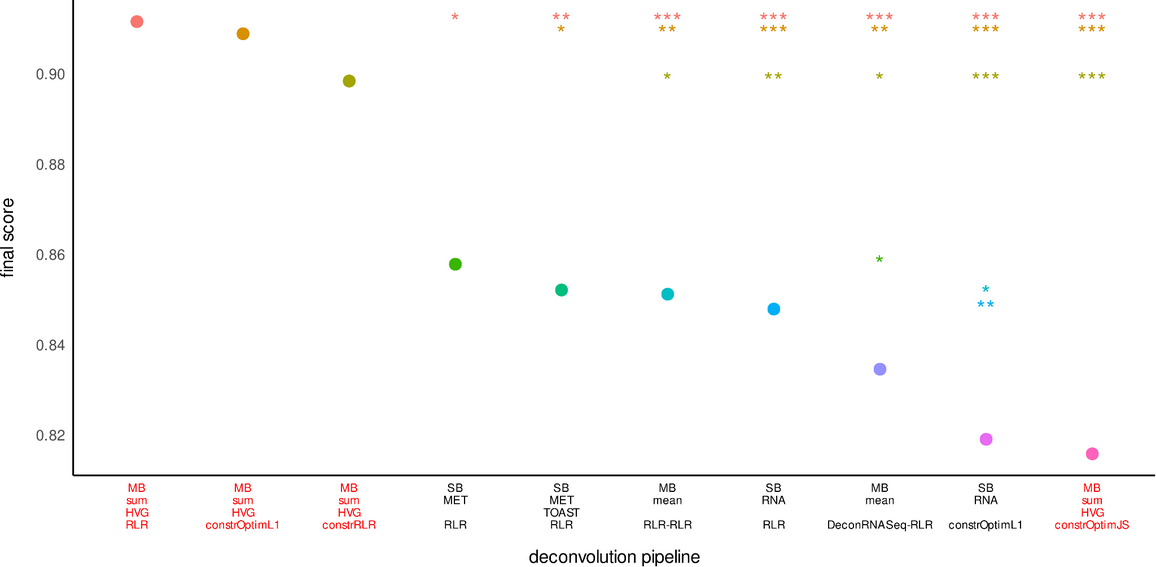
\includegraphics[width=\textwidth,keepaspectratio]{fig/sup_simu_topsignif.png}
    \caption{Top 10 deconvolution pipelines in the supervised setting, based on the final aggregated score computed on the simulated datasets. The red labels correspond to pipelines employing the summation integration. Stars correspond to the typical significance levels for the permutation test between pairs of pipelines.}
    \label{fig:sup_simu_topsignif}
\end{figure}

\begin{figure}[htp]
    \centering
    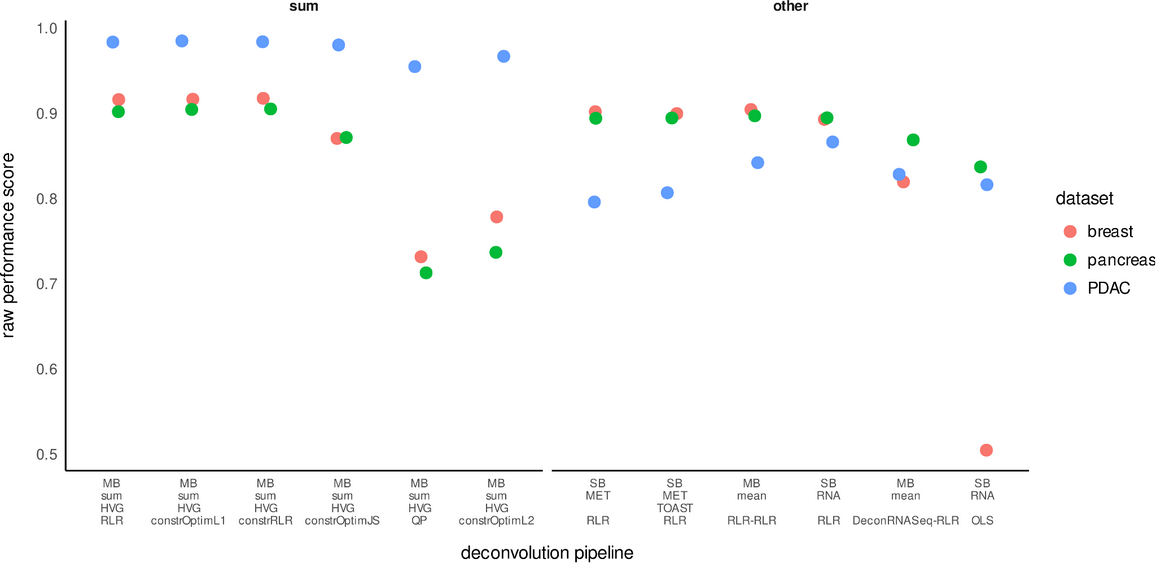
\includegraphics[width=\textwidth,keepaspectratio]{fig/sup_simu_sumtop.png}
    \caption{Intermediate scores per dataset and metric category on the simulated datasets of the summation-based integration pipelines, along with interesting alternative pipelines.}
    \label{fig:sup_simu_sumtop}
\end{figure}

In addition to the final ranking obtained after applying the aggregation method described in Section \ref{subsubsec:scoring-ranking}, the permutation test procedure presented in Section \ref{subsubsec:statistically-significant-performance-improvement} allows us to estimate the significance level of difference between two pipelines.
Figure \ref{fig:sup_simu_topsignif} shows that the best candidate is the one combining the RLR deconvolution with the early summation configuration described in Section \ref{subsubsec:early-integration}.
From this figure, we can also see that its final aggregated score is significantly larger (i.e. better) than the ones of all candidates outside of the top three.
Quite interestingly, all the top three candidates are based on the early summation integration!
Since their results are not significantly different according to our test, we can consider them as our benchmark \say{winners} and we could conclude that multi-omics strategy proves to be more efficient when using an early integration.

However, while it is very convenient to use a scores aggregation function to rank candidates, it does not allow to grasp understanding about why one candidate is better than others.
I did not had time to investigate the possible reasons behind the good performances of the early summation integration, but we can already see from Figure \ref{fig:sup_simu_sumtop} that all the pipelines based on this integration technique exhibit higher raw performances than the others on the simulated PDAC dataset, whereas their performance on the other datasets are not standing out.
Therefore, before concluding on the overall benefit of the summation integration as suggested by simply looking at the final score, additional investigations should be done.

\subsubsection{Or the unsupervised one}\label{subsubsec:results-unsupervised}

\begin{figure}[htp]
    \centering
    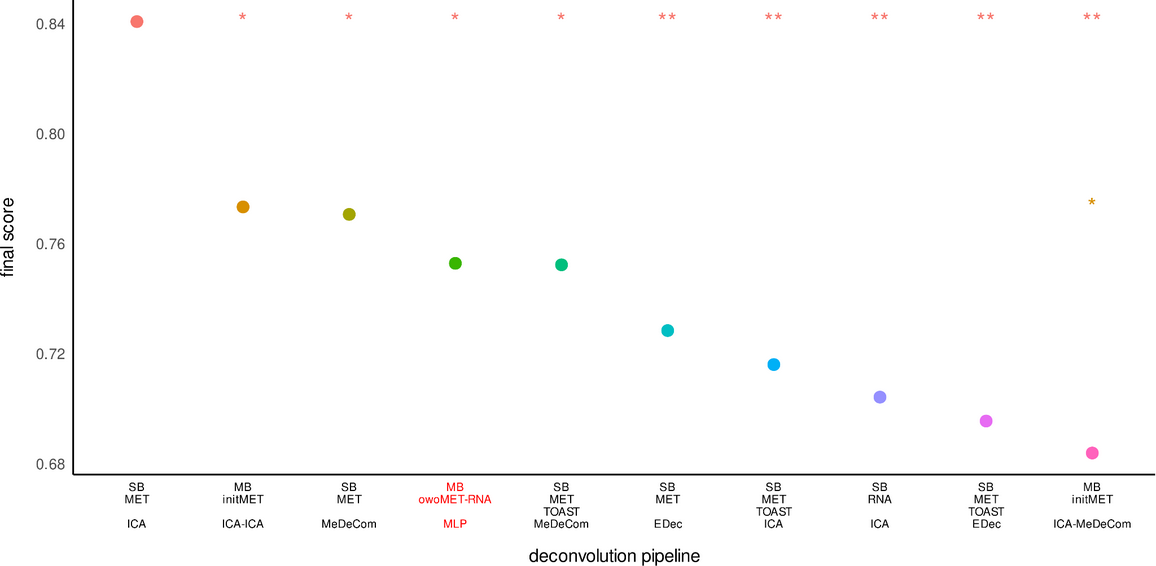
\includegraphics[width=\textwidth,keepaspectratio]{fig/unsup_simu_topsignif.png}
    \caption{Top 10 deconvolution pipelines in the unsupervised setting, based on the final aggregated score computed on the simulated datasets. Red labels highlight pipelines employing the VAE integration. Stars correspond to the typical significance levels of the permutation test between pairs of pipelines.}
    \label{fig:unsup_simu_topsignif}
\end{figure}

As with the supervised setting, we first observed the overall performance on the simulated dataset, assessed by the final aggregated score.
From Figure \ref{fig:unsup_simu_topsignif}, we can elect a clear \say{winner}, as applying ICA on raw methylome data provides a final score significantly larger than that of all the other methods when compared pairwise.
It is noteworthy that a majority of the top-performing pipelines utilize the methylome block, a trend that contrasts with the findings in the supervised scenario.
Only three MB deconvolution pipelines are present in the top 10, including one of the VAE-based approach described in Section \ref{subsubsec:intermediate-integration}.
In the unsupervised scenario, it seems that MB approaches, at least those we evaluated, do not yield improvements in the deconvolution task.

\begin{table}[ht]
\centering
\caption{OWO-VAE and TWO-VAE fitted hyperparameters.}
\label{tab:vae_hp_fitted}
\begin{tabular}{l|c|c|c|c}
 & $\lambda_1^*$ & $\lambda_3^*$ & $u_0^*$ & $k^*$ \\ \hline
MB two MLP & 1e-2 & 1e-4 & 100 & 2e-2 \\ \hline
MB owoMET-RNA MLP & 1e-2 & NA & 25 & 2e-2 \\ \hline
MB owoRNA-MET MLP & 1e-3 & NA & 25 & 2e-2 \\ \hline
SB owoMET MLP & 1e-4 & NA & 25 & 2e-2 \\ \hline
SB owoRNA MLP & 1e-3 & NA & 25 & 1e-2
\end{tabular}
\end{table}

\begin{figure}[htb]
    \centering
    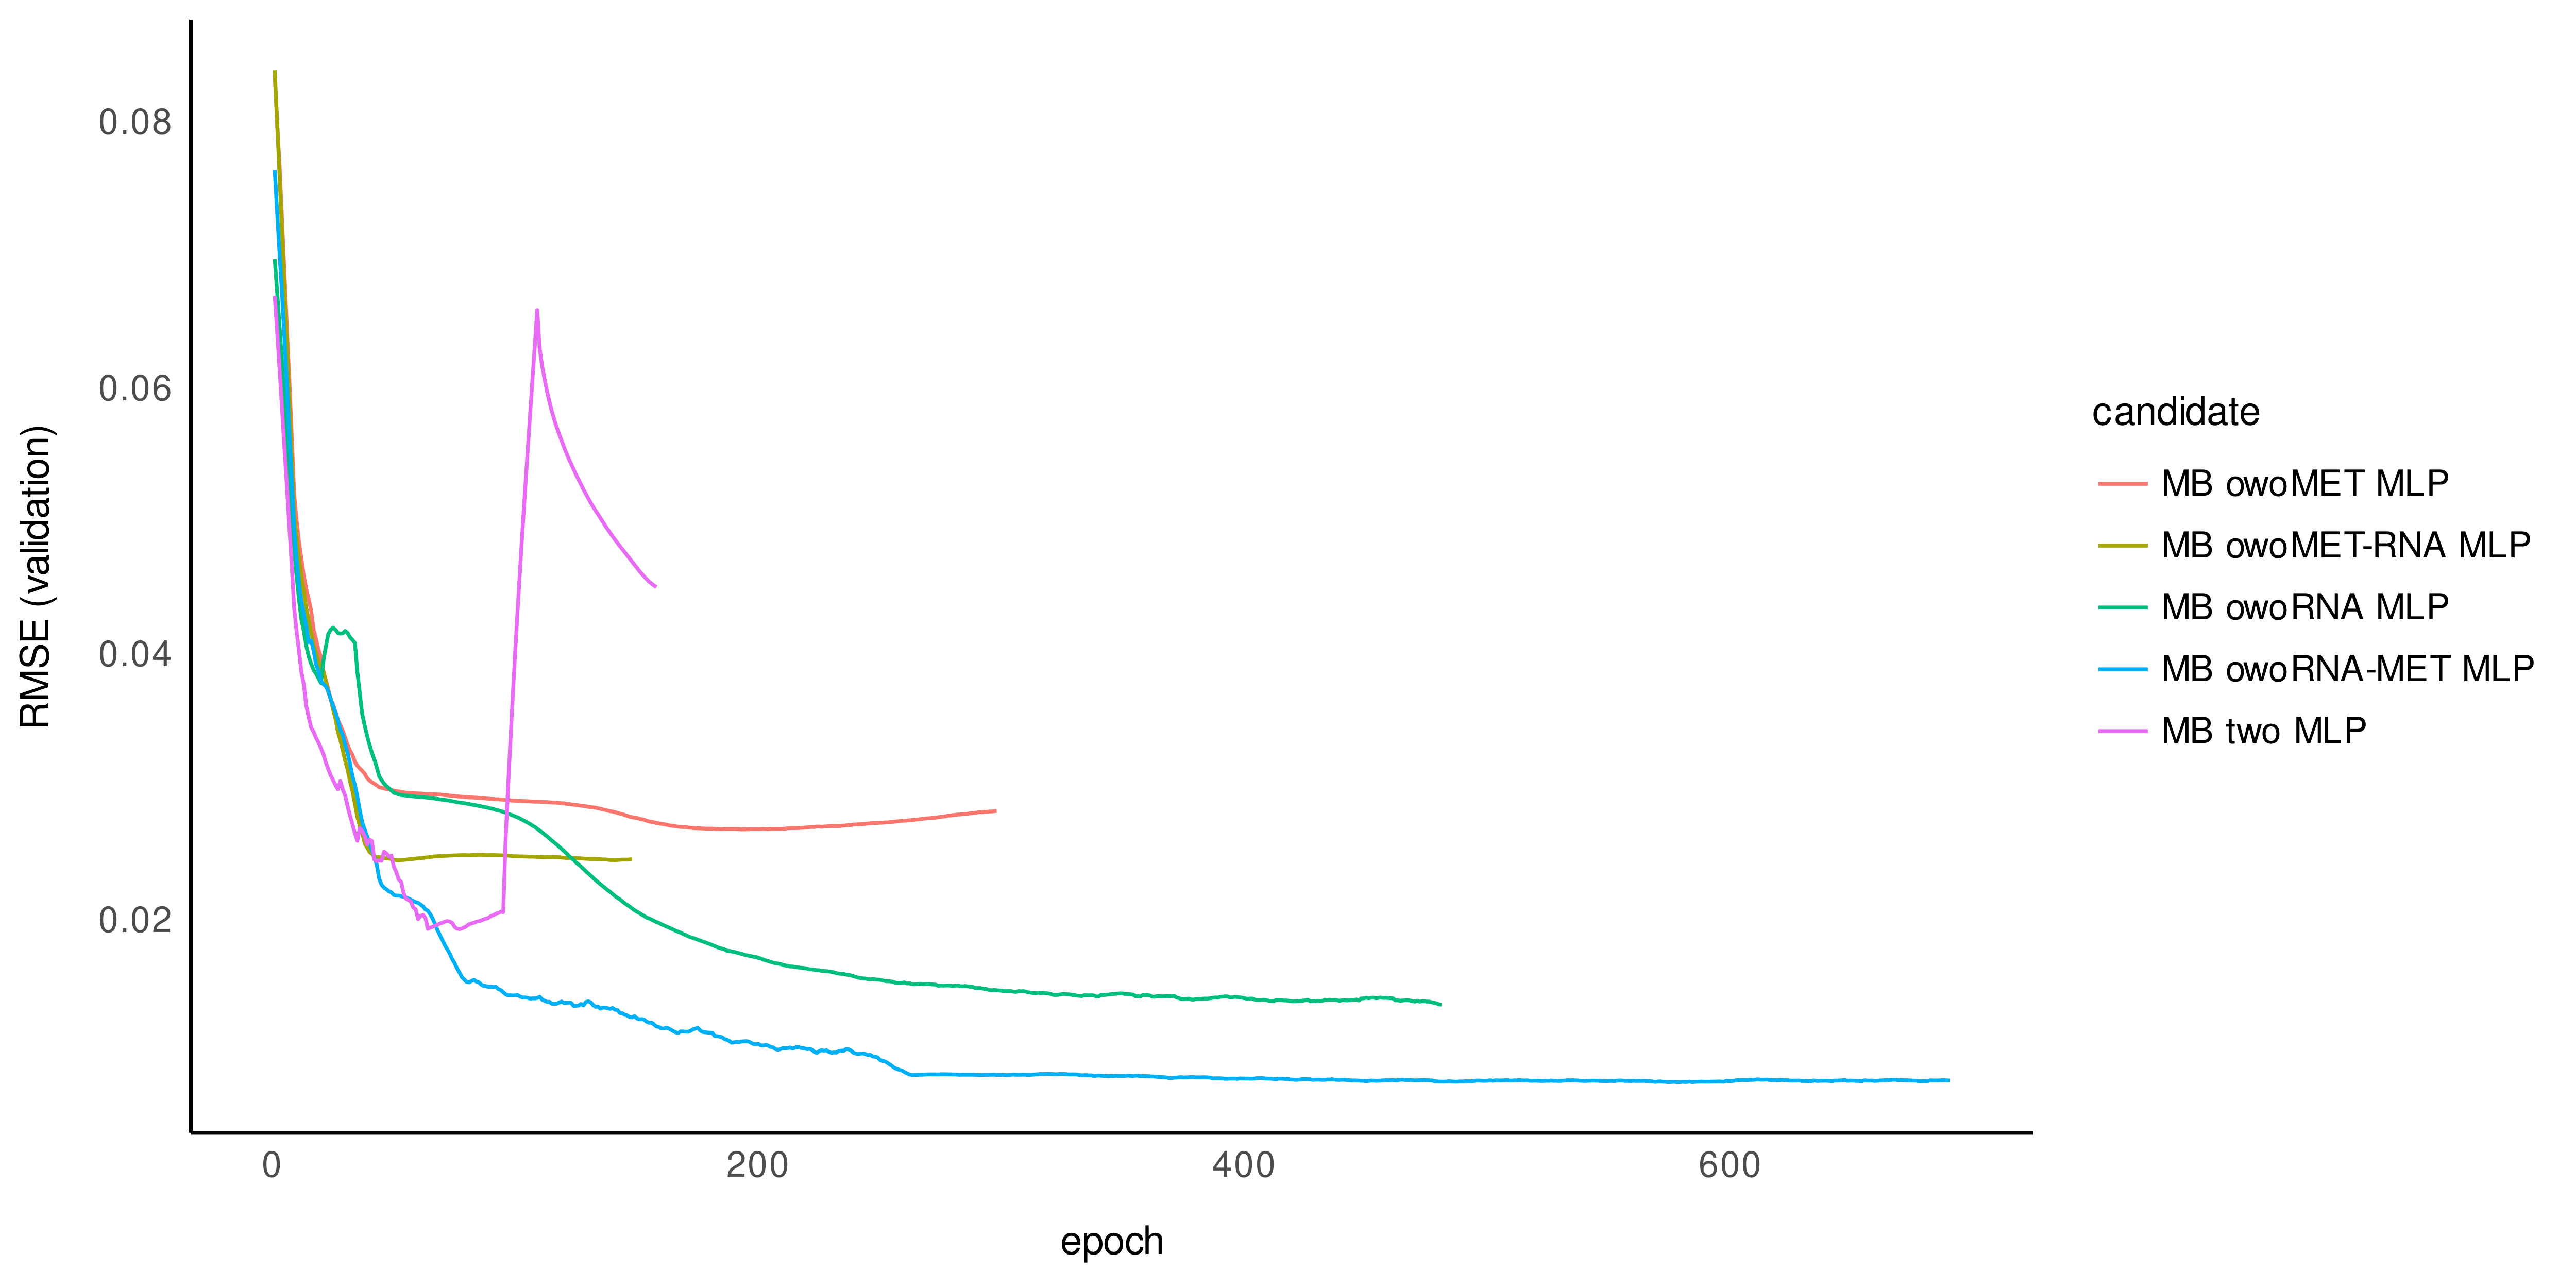
\includegraphics[width=\textwidth,keepaspectratio]{fig/vae_val_rmse.png}
    \caption{Evolution of the VAE-based pipelines: RMSE computed on the validation set over training epochs.}
    \label{fig:vae_val_rmse}
\end{figure}

Table \ref{tab:vae_hp_fitted} displays the optimal set of hyperparameters for the OWOs and TWO hyparameters.
Interestingly, the column $u_0^*$ indicates that the OWOs models exhibit improve performance with early regularization, while the TWO architecture benefits from a later one.
Given that $\lambda_3^*=\text{1e-4}$, it is possible that the OT term might not contribute to the optimization of network parameters.
Examining the evolution of the RMSE on the validation set over training epochs on Figure \ref{fig:vae_val_rmse}, it becomes apparent that the deconvolution performance of the \textit{MB two MLP} and \textit{MB owo MLP} models is affected upon the introduction of regularization.
The optimization of the \textit{MB owo MLP} model is moderately impacted, quickly able to find a new minimum increasing deconvolution performance.
However \textit{MB two MLP} appears to be more adversely impacted by the addition of the KL term to its loss function.
The optimization process was prematurely terminated by the scheduler before it could converge again to an optimum that favors the deconvolution task.
This situation raises questions regarding the introduction of regularization in this case.

\begin{figure}[htp]
    \centering
    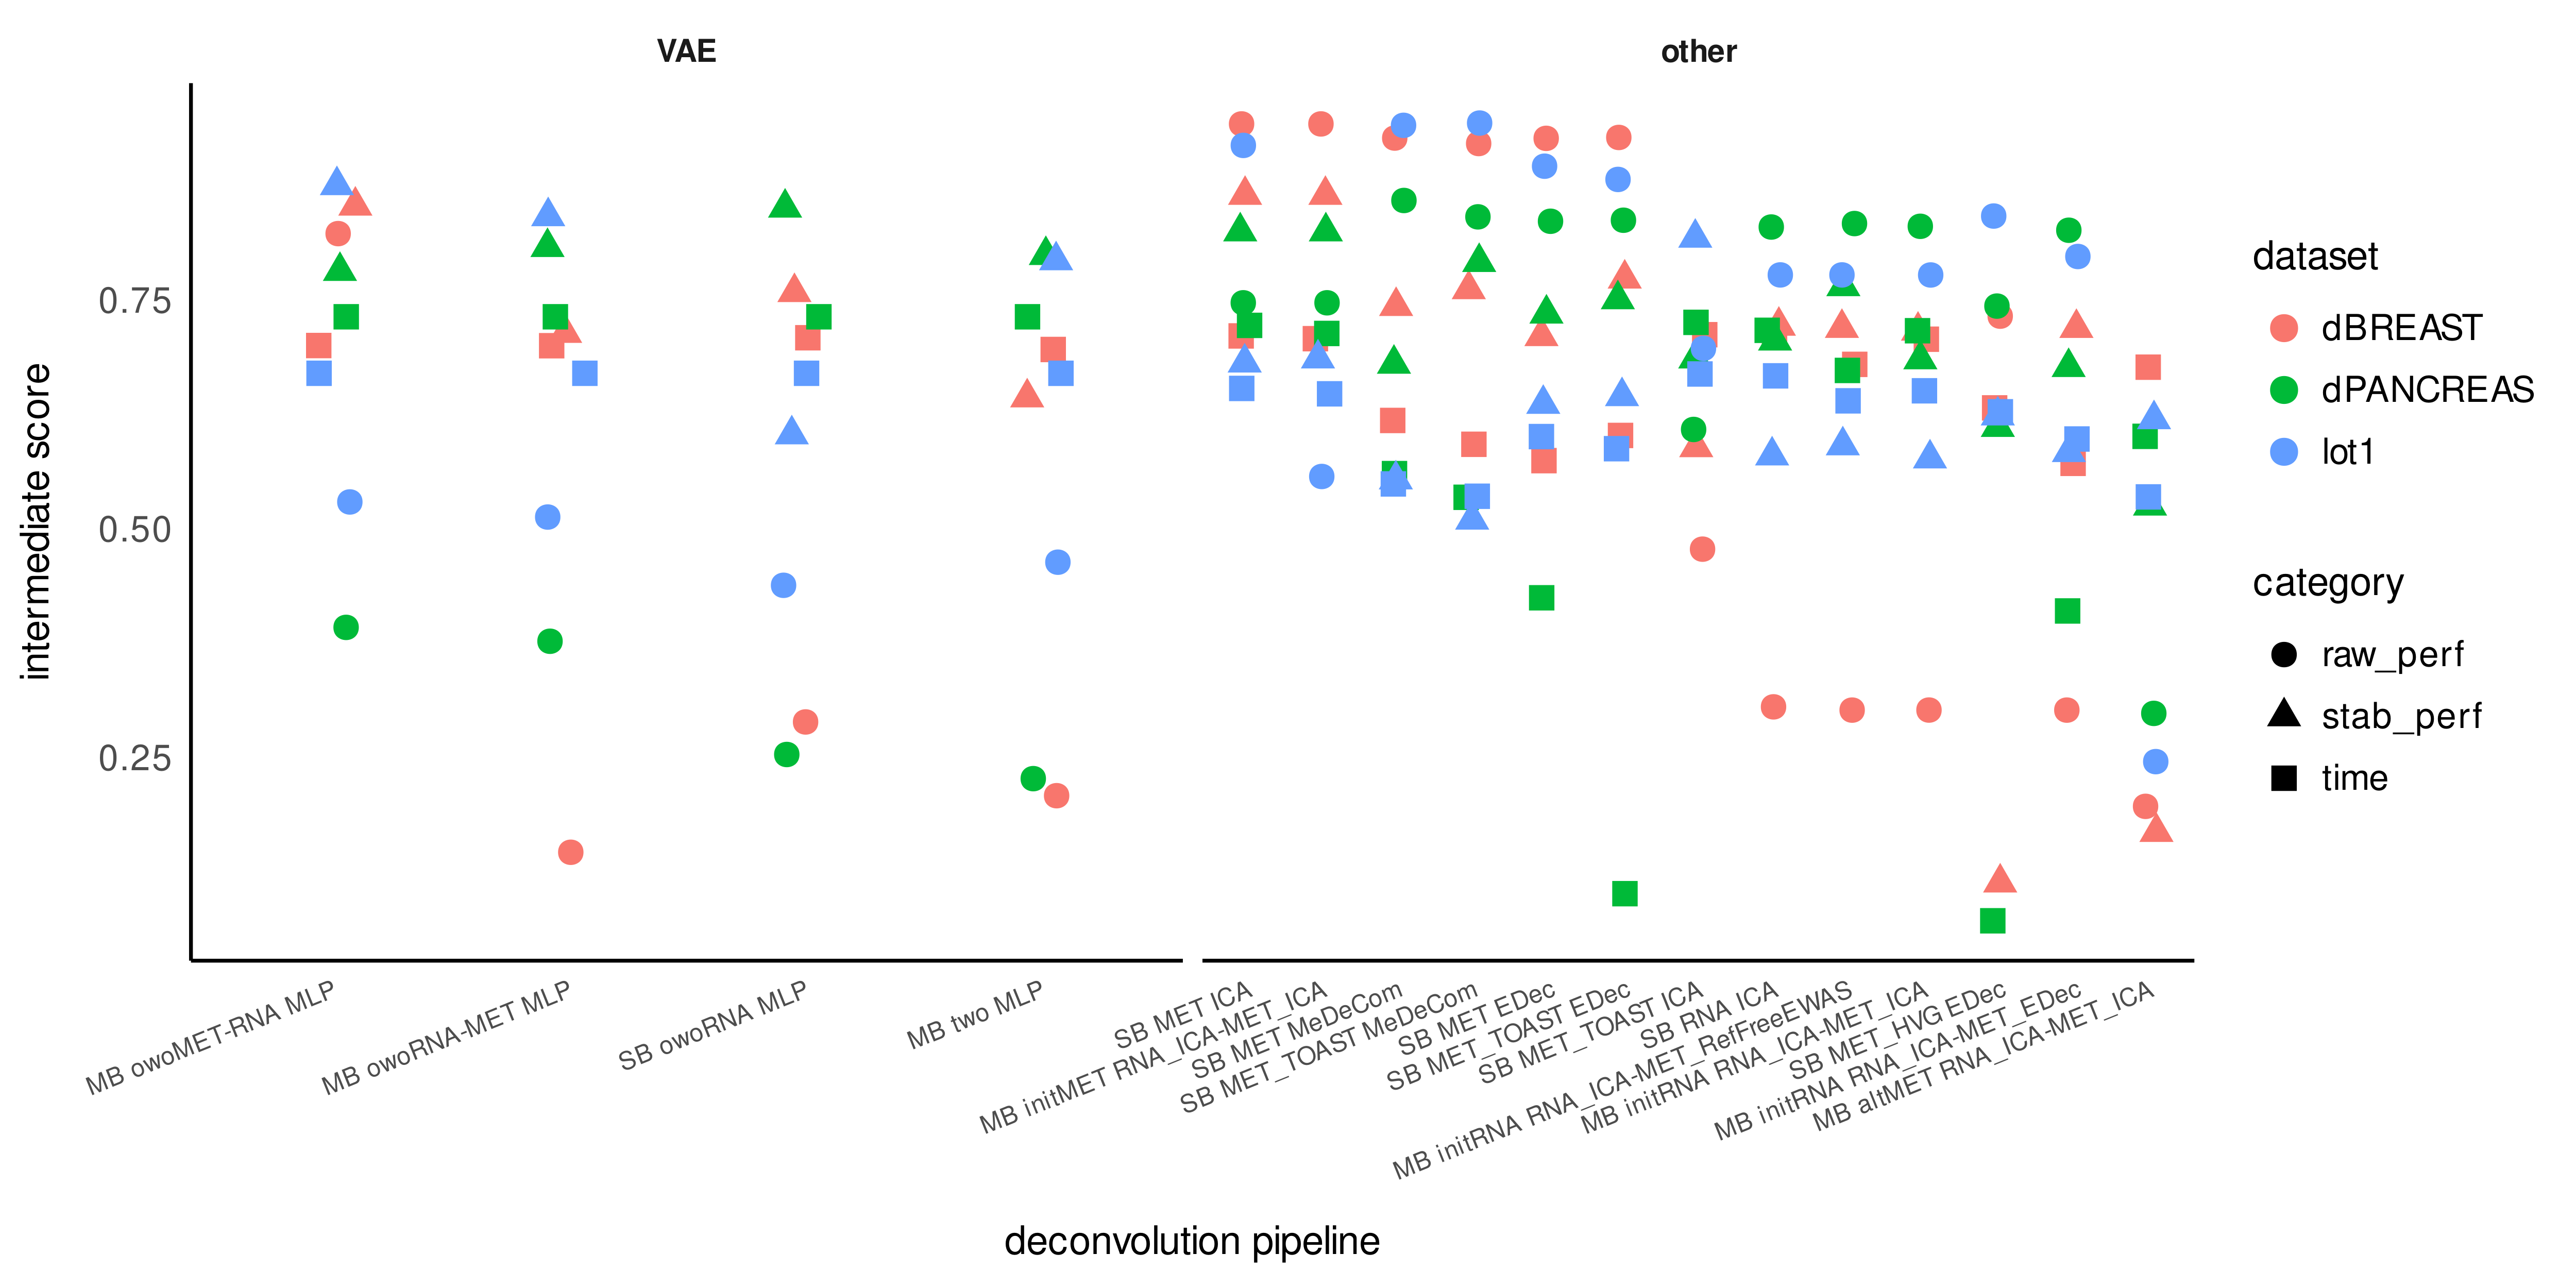
\includegraphics[width=\textwidth,keepaspectratio]{fig/unsup_simu_vaetop.png}
    \caption{Intermediate scores per dataset and metric category on the simulated datasets of the VAE-based integration pipelines, along with interesting alternative pipelines.}
    \label{fig:unsup_simu_vaetop}
\end{figure}

Although models optimization converges (leaving \textit{MB two MLP} aside), Figure \ref{fig:unsup_simu_vaetop} unmistakably highlights the generally poor raw deconvolution performance using the VAE integration.
Only the OWO model encoding from the methylome and decoding to the transcriptome demonstrated relatively good performance on the dataset simulating breast-like tumors.
Upon preliminary analysis, I observed that VAE models struggle to deconvolve according to all three sets of concatenated cell types.
Instead, the optimization process tends to \say{focus} on one of the sets.
Consequently, we should not expect decent deconvolution performances on more than one dataset at a time.
Addressing this challenge could involve constructing a more universally applicable set of cell types (knowing that it will not be an easy task because of tissue imprinting), or perhaps considering the use of models tailored to specific cancer types or subtypes.

\subsection{Assessing our benchmark robustness}\label{subsec:assessing-our-benchmark-robustness}

\subsubsection{Using the desired properties quantified with empirical criteria}

Returning to our objective of constructing a fair and comprehensive benchmark, we also used simulated datasets to compute the empirical criteria and characterize its behavior.
To understand if averaging three aggregations, as explained in Section \ref{subsubsec:scoring-ranking}, helps to this regard, we also computed those criteria for the three intermediate aggregations.
Figure \ref{fig:empirical_pavao} demonstrates that, both in the supervised and unsupervised settings, the elected winner exhibits good properties as it is very often ranked first when competing against other candidates (condorcet rate), and its normalized rank is nearly equal to 1.
However, the ranking process appears to be affected by judges' perturbation, as the generalization property is poorly preserved, with a mean correlation between the true and perturbed ranking being less than 0.6.

\begin{figure}[htp]
    \centering
    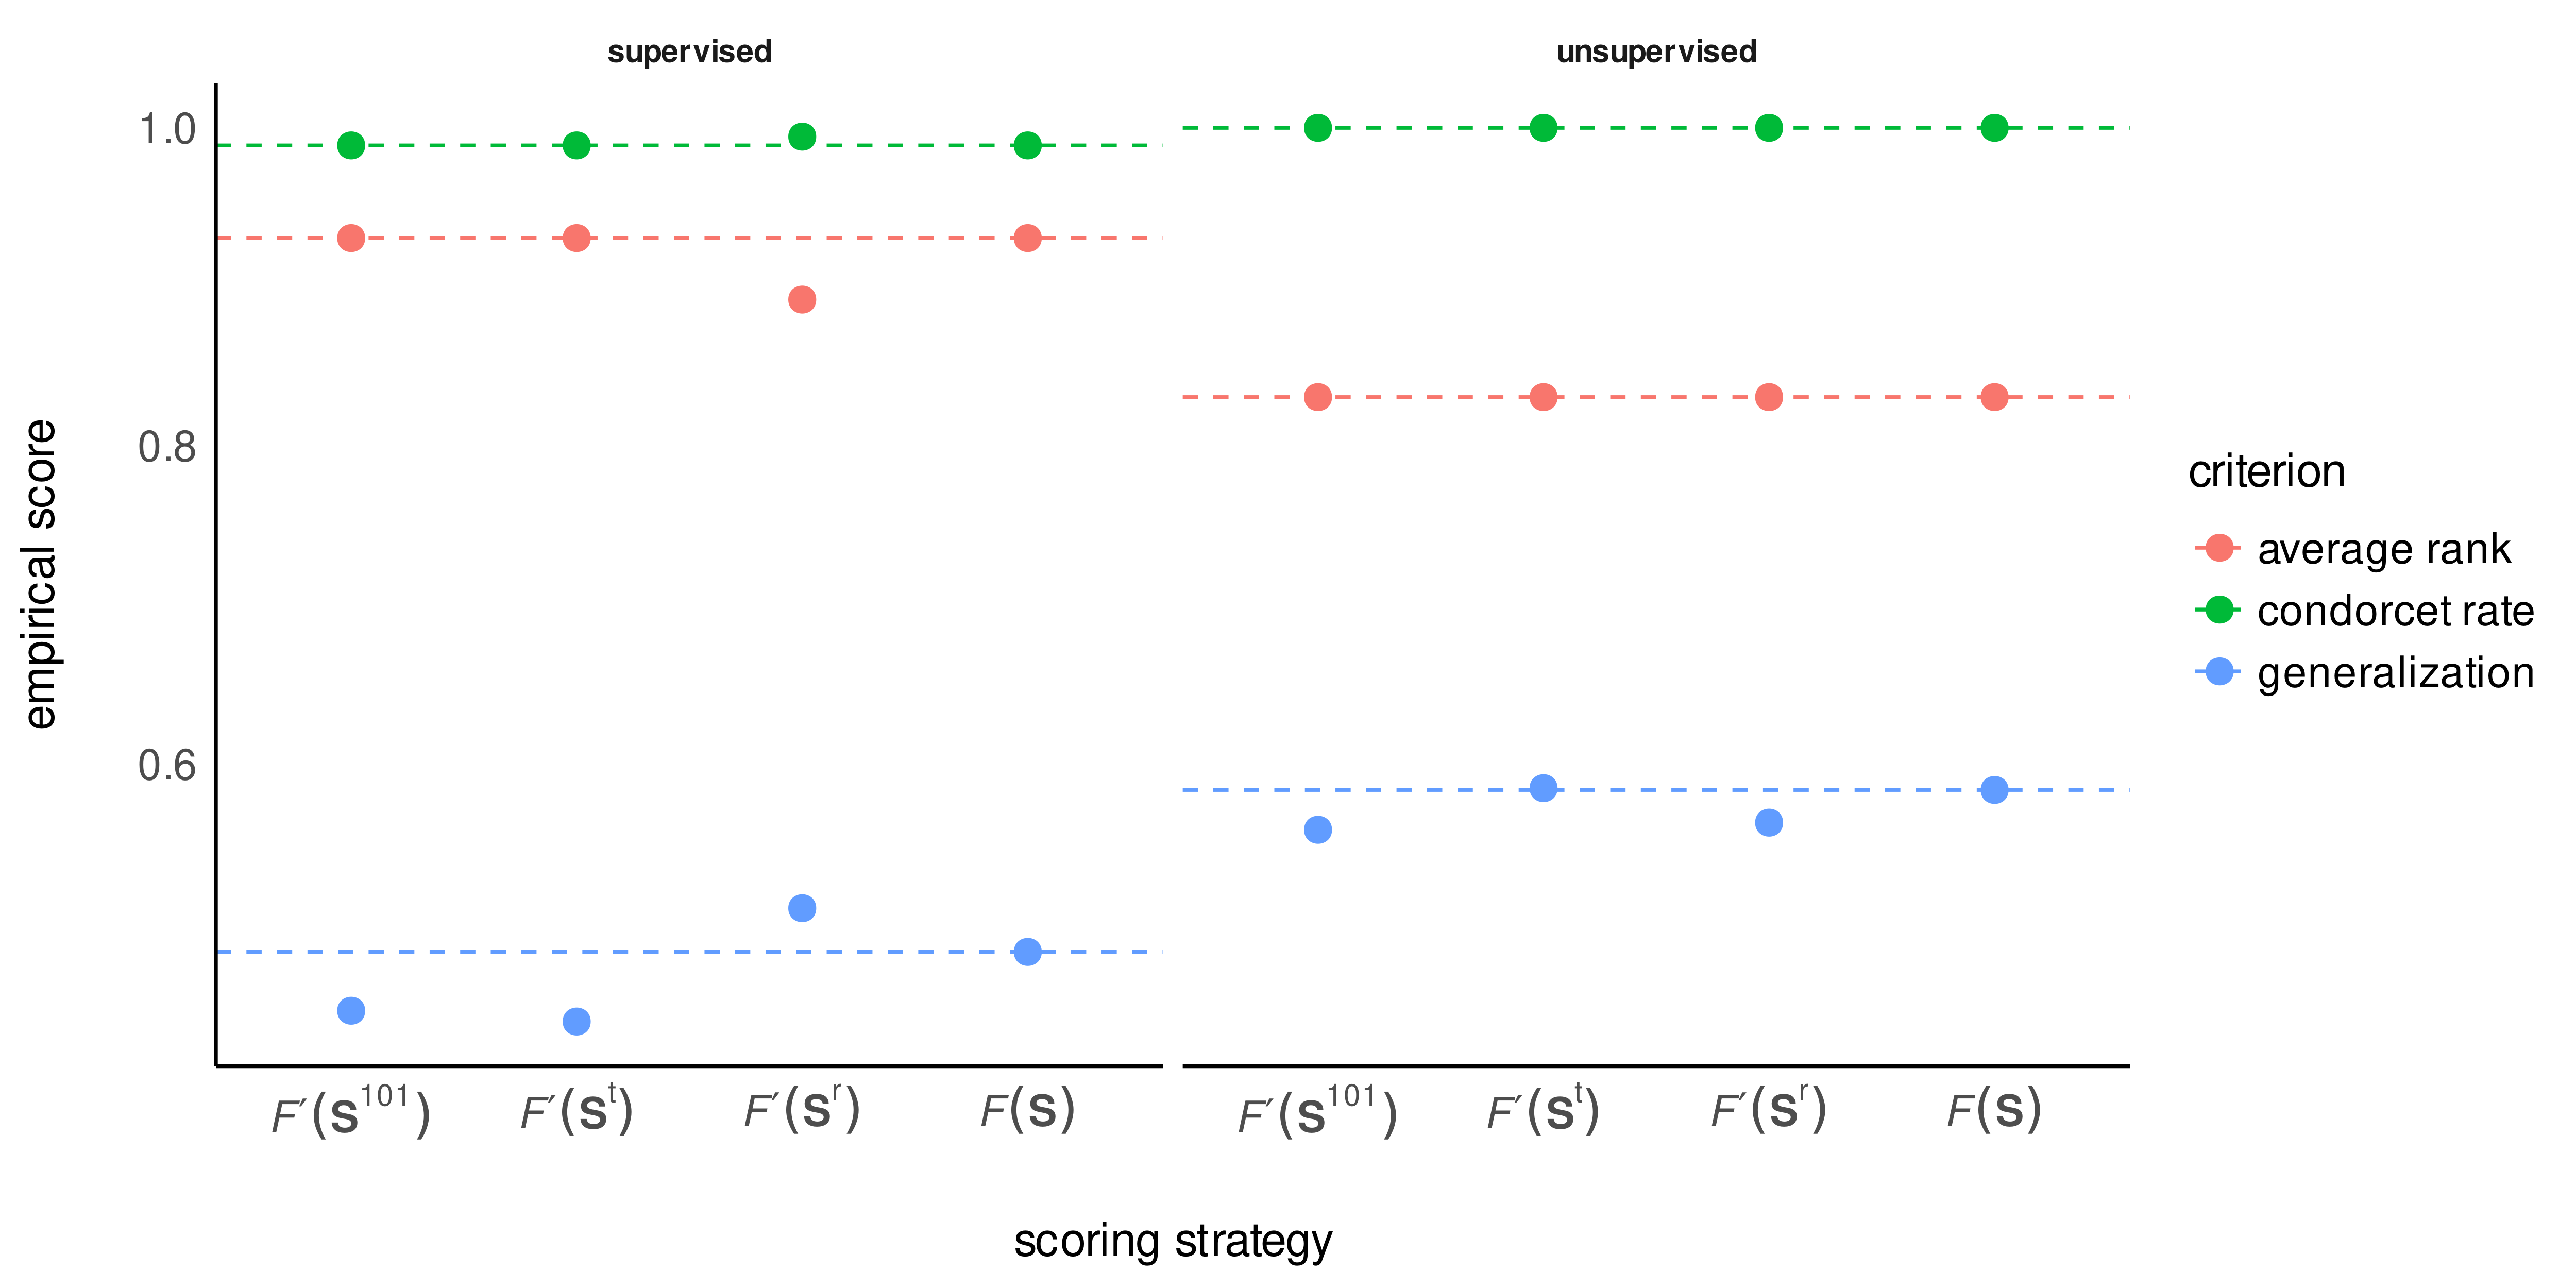
\includegraphics[width=\textwidth,keepaspectratio]{fig/empirical_pavao.png}
    \caption{Empirical evaluation of desired ranking properties in both supervised and unsupervised settings. Dashed lines correspond the scores of the ranking strategy $\mathcal{F}(\mathbf{S})$.}
    \label{fig:empirical_pavao}
\end{figure}

Overall, the empirical scores of the ranking strategy $\mathcal{F}(\mathbf{S})$ suggest that it benefits from the good properties of the others, while not being impacted by their poorer ones.
In fact, from Table \ref{tab:pavao_topsis} showing the TOPSIS similarity, computed using the three empirical criteria, of the four ranking strategies, $\mathcal{F}(\mathbf{S})$ appears to be the ideal solution.
However, is the TOPSIS similarity the appropriate ranking method for this, especially since in this case $\mathcal{F'}(\mathbf{S}^t)$ performed badly?
The issue of determining the ultimate ranking strategy circles back upon itself, ultimately leading us to rely on the belief that our chosen approach is reasonable.  

\begin{table}[ht]
\centering
\caption{TOSIS similarity of the aggregation functions.}
\label{tab:pavao_topsis}
\begin{tabular}{c|c|c|c}
$\mathcal{F}(\mathbf{S})$ & $\mathcal{F'}(\mathbf{S}^r)$ & $\mathcal{F'}(\mathbf{S}^t)$ & $\mathcal{F'}(\mathbf{S}^{101'})$ \\ \hline
0.90 & 0.75 & 0.38 & 0.25
\end{tabular}
\end{table}

\subsubsection{And our in vitro PDAC dataset}

Considering that the in vitro dataset of PDAC tumors was not employed in constructing the rankings presented in Section \ref{subsec:do-multi-omics-strategies-perform-better?}, it can be viewed as a fresh set of evaluators for our candidate pipelines.
With this perspective, the results on the in vitro PDAC dataset can also shed light on the robustness of the benchmark.
Table \ref{tab:simu_real_comp} outlines the rankings of the top supervised and unsupervised deconvolution pipelines across both simulated datasets and the in vitro PDAC dataset.
The \textit{NA} values in the table represent cases where pipelines encountered numerical errors while attempting the deconvolution.

In the supervised setting, the summation-based candidates maintain their strong performance on the in vitro PDAC dataset.
Interestingly, some of these pipelines were not originally ranked as high in the benchmark on simulated data.
This discrepancy can be attributed to the insight shared in Section \ref{subsubsec:results-supervised}: their raw performances were notably superior on the simulated PDAC dataset.
Conversely, there is a group of methods that were reasonably well ranked on the simulated datasets but have now dropped in ranking on in vitro data.
Figure \ref{fig:sup_simu_sumtop} continues to offer insights into this phenomenon, as these pipelines did not demonstrate noteworthy performance on the simulated PDAC dataset.

Differences in rankings observed in the unsupervised scenario are more challenging to interpret due to a significant portion of the top-performing pipelines on the simulated datasets not successfully running on the in vitro PDAC dataset.
Consequently, there is a strong possibility that many methods experienced an artificial boost in ranking.
The significant jump of the TWO-based integration candidate from the 23rd position to the 2nd position requires thorough investigation, especially considering that its performances on the simulated PDAC dataset were only average, as shown in Figure \ref{fig:unsup_simu_vaetop}, and that its learning curve plotted in Figure \ref{fig:vae_val_rmse} was not at all promising.

\begin{table}[ht]
\centering
\caption{Ranks of the best deconvolution pipelines achieved on both the simulated datasets and the real dataset. Pipelines employing summation or VAE integration are highlighted in red.}
\label{tab:simu_real_comp}
\resizebox{\textwidth}{!}{
\begin{tabular}{l|cc||l|cc}
 & \multicolumn{2}{c||}{Ranks} & & \multicolumn{2}{c}{Ranks} \\
Supervised pipelines & simulated & real & Unsupervised pipelines & simulated & real \\ \hline
\color[HTML]{CB0000} MB sum\_HVG RLR & \cellcolor[HTML]{F0F921} 1 & \cellcolor[HTML]{F1F426} 3 & SB MET ICA & \cellcolor[HTML]{F0F921} 1 & \cellcolor[HTML]{F1F426} 3 \\ 
\color[HTML]{CB0000} MB sum\_HVG constrRLR & \cellcolor[HTML]{F1F426} 3 & \cellcolor[HTML]{F0F624} 2 & \color[HTML]{CB0000} MB owoMET-RNA MLP & \cellcolor[HTML]{F1F426} 3 & \cellcolor[HTML]{F2F227} 4 \\ 
\color[HTML]{CB0000} MB sum\_HVG constrOptimL1 & \cellcolor[HTML]{F0F624} 2 & \cellcolor[HTML]{F2F227} 4 & SB RNA ICA & \cellcolor[HTML]{F5E926} 8 & \cellcolor[HTML]{F0F921} 1 \\ 
\color[HTML]{CB0000} MB sum\_HVG QP & \cellcolor[HTML]{F7E525} 10 & \cellcolor[HTML]{F0F921} 1 & MB initRNA RNA\_ICA-MET\_ICA & \cellcolor[HTML]{F7E225} 11 & \cellcolor[HTML]{F3F027} 5 \\ 
\color[HTML]{CB0000} MB sum\_HVG constrOptimJS & \cellcolor[HTML]{F6E826} 9 & \cellcolor[HTML]{F3EE27} 6 & SB MET EDec & \cellcolor[HTML]{F2F227} 4 & \cellcolor[HTML]{F8DE25} 13 \\ 
\color[HTML]{CB0000} MB sum\_HVG constrOptimL2 & \cellcolor[HTML]{F8E125} 12 & \cellcolor[HTML]{F3F027} 5 & MB initRNA RNA\_ICA-MET\_RefFreeEWAS & \cellcolor[HTML]{F8DE25} 13 & \cellcolor[HTML]{F3EE27} 6 \\ 
SB RNA OLS & \cellcolor[HTML]{FCCF25} 20 & \cellcolor[HTML]{F7E525} 10 & \color[HTML]{CB0000} MB owoRNA-MET MLP & \cellcolor[HTML]{F8E125} 12 & \cellcolor[HTML]{F5E926} 8 \\ 
SB RNA RLR & \cellcolor[HTML]{F5EC27} 7 & \cellcolor[HTML]{FDC727} 24 & \color[HTML]{CB0000} SB owoRNA MLP & \cellcolor[HTML]{FADA24} 15 & \cellcolor[HTML]{F5EC27} 7 \\ 
MB mean RNA\_DeconRNASeq-MET\_RLR & \cellcolor[HTML]{F5E926} 8 & \cellcolor[HTML]{FCA835} 40 & \color[HTML]{CB0000} MB two MLP & \cellcolor[HTML]{FDCA26} 23 & \cellcolor[HTML]{F0F624} 2 \\ 
SB MET\_TOAST RLR & \cellcolor[HTML]{F3F027} 5 & \cellcolor[HTML]{F58C46} 56 & MB initRNA RNA\_ICA-MET\_EDec & \cellcolor[HTML]{FBD324} 18 & \cellcolor[HTML]{F7E525} 10 \\ 
MB mean RNA\_RLR-MET\_RLR & \cellcolor[HTML]{F3EE27} 6 & \cellcolor[HTML]{F3864A} 59 & MB altMET RNA\_ICA-MET\_ICA & \cellcolor[HTML]{FEBB2B} 30 & \cellcolor[HTML]{F6E826} 9 \\ 
SB MET RLR & \cellcolor[HTML]{F2F227} 4 & \cellcolor[HTML]{EE7B51} 66 & MB initMET RNA\_ICA-MET\_ICA & \cellcolor[HTML]{F0F624} 2 & NA \\ 
SB RNA\_TOAST OLS & \cellcolor[HTML]{CB4679} 101 & \cellcolor[HTML]{F6E826} 9 & SB MET MeDeCom & \cellcolor[HTML]{F3EE27} 6 & NA \\ 
SB RNA SVR & \cellcolor[HTML]{AD2793} 123 & \cellcolor[HTML]{F5EC27} 7 & SB MET\_TOAST EDec & \cellcolor[HTML]{F3F027} 5 & NA \\ 
SB RNA\_TOAST NNLS & NA & \cellcolor[HTML]{F5E926} 8 & SB MET\_TOAST ICA & \cellcolor[HTML]{F6E826} 9 & NA \\ 
 &  &  & SB MET\_TOAST MeDeCom & \cellcolor[HTML]{F5EC27} 7 & NA \\ 
 &  &  & SB MET\_HVG EDec & \cellcolor[HTML]{F7E525} 10 & NA
\end{tabular}
}
\end{table}

\section{Conclusion}\label{sec:conclusion}

Over the course of this internship, I have achieved several milestones that, I hope, have contributed to the advancement of the Acacia project and the team's effort in the field of deconvolution pipelines and integration strategies.
Let's delve into those accomplishments, the future possibilities they open, and my key takeaways from this work.

\subsection{Achievements}\label{subsec:achievements}

We constructed and ran a comprehensive benchmark to evaluate deconvolution pipelines.
This benchmark encompassed around 190 candidates, spanning both multi-block (MB) and single-block (SB) approaches.
The evaluation was conducted on simulated datasets mimicking three distinct types or subtypes of cancer: breast, pancreatic, and PDAC.
The ranking of candidates encompassed a comprehensive assessment based on three distinct performance metrics: raw performance, performance stability, and computation time.
I proposed a permutation test procedure to determine the significance of improvement between pairs of candidates.
Furthermore, performances of the deconvolution candidates on simulated data were compared with the ones on a real, in vitro, PDAC dataset.

Additionally, I introduced and evaluated two novel MB integration strategies.
The first approach involved early summation of omic blocks, followed by several supervised deconvolution tools.
The second approach, combining VAE and MLP in an end-to-end DL framework belongs to the intermediate integration timing and the unsupervised deconvolution.

To ensure a fair comparison among all the pipelines, I established and utilized a stable and easily reproducible software environment. 
I then ran the benchmark on the reliable hardware of the GRICAD infrastructure.

On a more personal note, I presented a poster (see Appendix \ref{app:poster}) addressing benchmark construction, scoring strategy, and the permutation test procedure at JOBIM and ISMB conferences.

\subsection{Outlook}\label{subsec:outlook}

There is certainly ample room for future work across various aspects of this project.

Concerning the summation-based approach, instead of summing features from the two blocks at random, it could be interesting to sum features that are biologically related, possibly duplicating transcriptomic features to account for the N-to-1 relation between genes and CpG sites.
Furthermore, investigating into the encouraging performance of this approach on the in vitro PDAC dataset could provide a deeper understanding of its potential. 
The prospect of employing the summed block with unsupervised deconvolution also holds promise, deserving exploration.

Regarding the VAE-based integration, there are potential avenues for enhancing its effectiveness. 
These include pursuing a unified cell types set and expanding training to cover a broader range of common input features across different cancer types and subtypes. 
The regularization process could be refined by transforming the gradual increase of the regularization weight into a more effective warm-up phase. 
This involves keeping the learning rate constant and disabling the early stopping scheduler, especially as deconvolution performance tends to temporarily degrade during regularization initiation.
Moreover, optimizing the regularization on the shared latent space of the TWO-VAE, rather than on individual OWO-VAEs, holds the potential for added benefits. 
Exploring the removal of regularization altogether and considering classical Autoencoders (AE) might also be valuable, given that our goal is not to generate posterior samples, but solely to perform deconvolution. 
Additionally, the question of whether to include training time in the performance evaluation remains open.
Same as for the summation approach, it could be interesting to explore the use of a VAE-based integration technique within the supervised setting by projecting the cell type references onto the learned latent space. 
Lastly, as architectures become more complex, the interpretability of their results also become challenging; if promising deconvolution performances are to be achieved, exploring this aspect becomes of significant importance.

More integration methods based on graph representations hold potential for fusing multi-omics.
I already mentioned GNN, but multi-layer networks, such as MultiXrank \cite{MultiXrank}, are also to be considered.

A pan-cancer approach could further enhance the comprehensiveness of the benchmark by including additional datasets, both simulated and in vitro, that cover a broader spectrum of cancer types and subtypes.

Finally, confronting benchmark results against datasets coming from cohorts of patients is a crucial validation step. 

\subsection{Key takeaways}

I really appreciated the reflection conducted on the robustness and comprehensiveness of benchmarks.
Based on the limited experience I gained during the internship, I would like to highlight two key points:
\begin{itemize}
    \item We observed the dilemma of selecting a ranking strategy based on empirical criteria.
    In the light of this, it has been crucial to revisit theoretical properties and design a ranking that aligns both with them and our benchmark's unique characteristics.
    \item While an aggregated score serves as a useful tool to offer an overall insight into candidates' performances, reverting to atomic scores is essential to understand the individual strengths and weaknesses of each candidate.
\end{itemize}

\clearpage

\printbibliography[heading=bibintoc,title={References}]

\clearpage

\titlespacing*{\section}{20pt}{-20pt plus 0pt minus 0pt}{-40pt plus 0pt minus 0pt}
\setlength{\headsep}{0pt}
\appendix
\section{Poster}\label{app:poster}
\begin{figure}[h!]
    \centering
    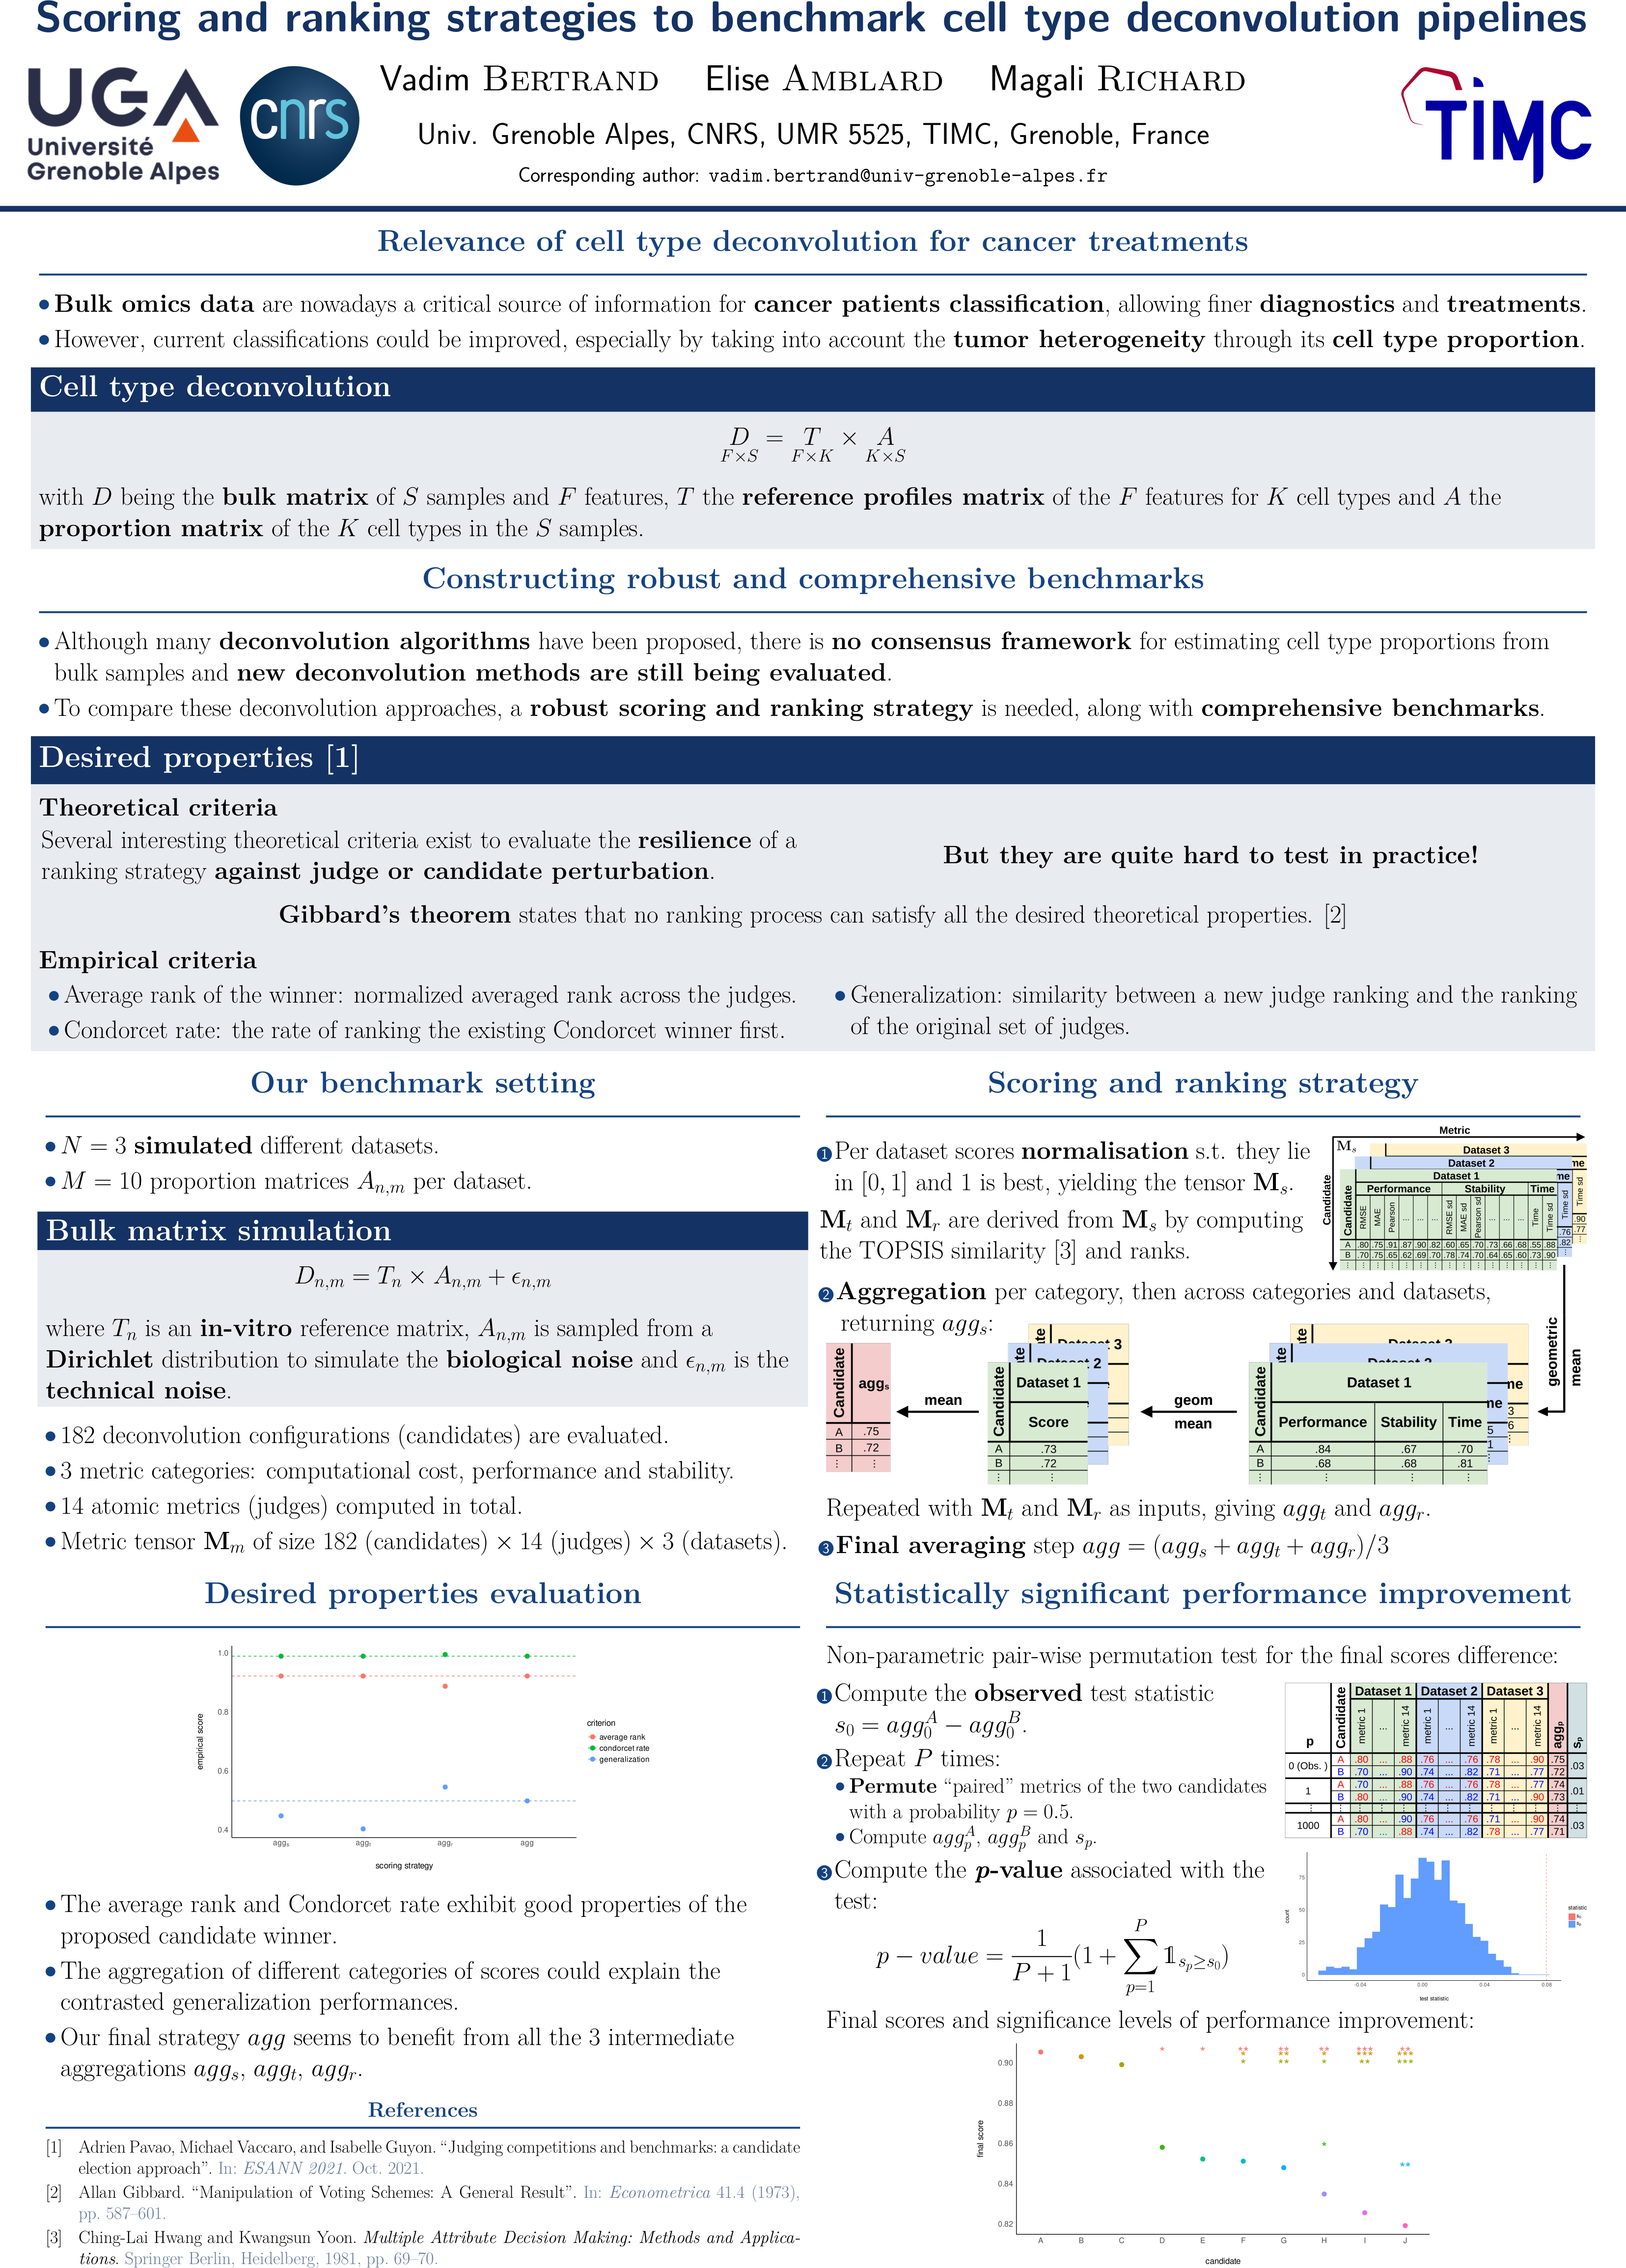
\includegraphics[height=20.3cm,keepaspectratio]{fig/poster.png}
\end{figure}
\setlength{\footskip}{0pt}

\end{document}